\chapter{Real-time $360 ^{\circ} $ cars rendering from multiple images with Gaussian Splatting}
\label{chapter:gausssplat}

\chapterwithfigures{\nameref*{chapter:gausssplat}} 
\chapterwithtables{\nameref*{chapter:gausssplat}}

\ifthenelse{\boolean{skipGauss}}{\endinput}{}

While 3D reconstruction landscape in deep learning has been entirely reshaped over the last few years with the \ac{NeRF} based framework, such technology remain ineffective for any industrial applications, both from a training (expressed in hours or even days) and inference perspective(regarding the milions of network queries required to render an image). \ac{GS} methods recently appeared as a well balanced trade-off between rendering quality and training/inference requirements. Contrary to \ac{NeRF} based methods, \ac{GS} does not rely on any neural network architecture. We propose through this last chapter a system that stabilised an unbounded scene depicting a single car to perform a stabilized $360 ^{\circ} $ rendering. We highlight in which extend such a learning-based method is better than a full image wrapping pipeline and develop the different modules we plugged in our pipeline to reach the best rendering quality as possible. Our experiments and corresponding ablation studies extensively confirm that such a pipeline is efficient for an industrial application. 

\section{Introduction}
This final chapter extends the latest two ones that were mostly focused toward a research academic perspective. Core motivation rather lies here on the desire to apply \ac{NVS} latest advances on an industrial project, where processed images resolution are at least $10\times$ higher than ShapeNet-SRN \citep{chang2015shapenet,sitzmann2019scene} ones ($\sim$ 1-2K against $128\times128$). \ac{NeRF} have benefited over the latest few years from massive improvements against several directions; training time, camera pose requirements, inference speed, drastic model weight reduction \textit{etc}. 
However, \ac{NeRF}-based methods suffers from an intrinsic computational bottleneck at inference time. It requires to query the \ac{NeRF} roughly 500 millions times to generate a squared $2K\times2K$ image. As a direct consequence, one of the most acknowledged state-of-the-art method, termed Mip-NeRF360 \citep{barron2022mip}, is only able to render at < 0.1 \ac{FPS} a 1K image. It would therefore be necessary to deploy a lot of \ac{GPU} resources and engineering refactorization to properly parallelize the source code in order to synthesize novel views at acceptable speed. 

We thus work in this last chapter with a different set of constraints. First concerns the generalizable property we kept in the two previous sections. We do not aim anymore to build or rely on an algorithm that can synthesize a viewpoint from any image belonging to a specific class. We thus rather want to leverage on \textit{per-scene} framework, that would require a novel training as soon as we work with a new scenario. Furthermore and as mentioned earlier, images we are now working with are closer to what clients could sent to any \ac{AI}-vision SaS company, both regarding resolution and content. Finally, camera poses are no longer available as ground truth since images CarCutter by Meero has to deal with are unposed. They thus must be first estimated using \ac{SFM} techniques.

Core idea is rather to leverage on the very latest advances in neural rendering, mostly on \ac{GS} ones. Contrary to \ac{NeRF}-based methods, that are therefore often too slow to render high-resolution images, \ac{GS} shows an impressive 100 \ac{FPS} performance, withtout relying on any neural network architecture. However, the \ac{NVS} paradigm we were used to deal with until now has heavely changed: View synthesis is not anymore infered given a source image and a camera transformation. As soon as \ac{GS} reconstructs the whole 3D scene through a set of 3D colored gaussians, render a novel view now at a specific viewpoint only require a camera pose information.

%%%%%%%%%%%%%
%%%%%%%%%%%%
We present on the Figure \ref{fig:gs-vs-homography-view3} how one of the view from the original image set as been stabilized by solely leveraging on image perspective wrapping (center image in Figure \ref{fig:gs-vs-homography-view3}). The same rendered view from the learned \ac{GS} scene is depicted on the right side of Figure \ref{fig:gs-vs-homography-view3}. As the entire 3D scene structure has been learned and is explicitly stored as a gaussian point cloud, one can render it at any locations and synthesise the whole car. The shown rendering comes from the vanilla \ac{GS} framework, without any of our modifications.

\begin{figure*}[htb!]
  \center
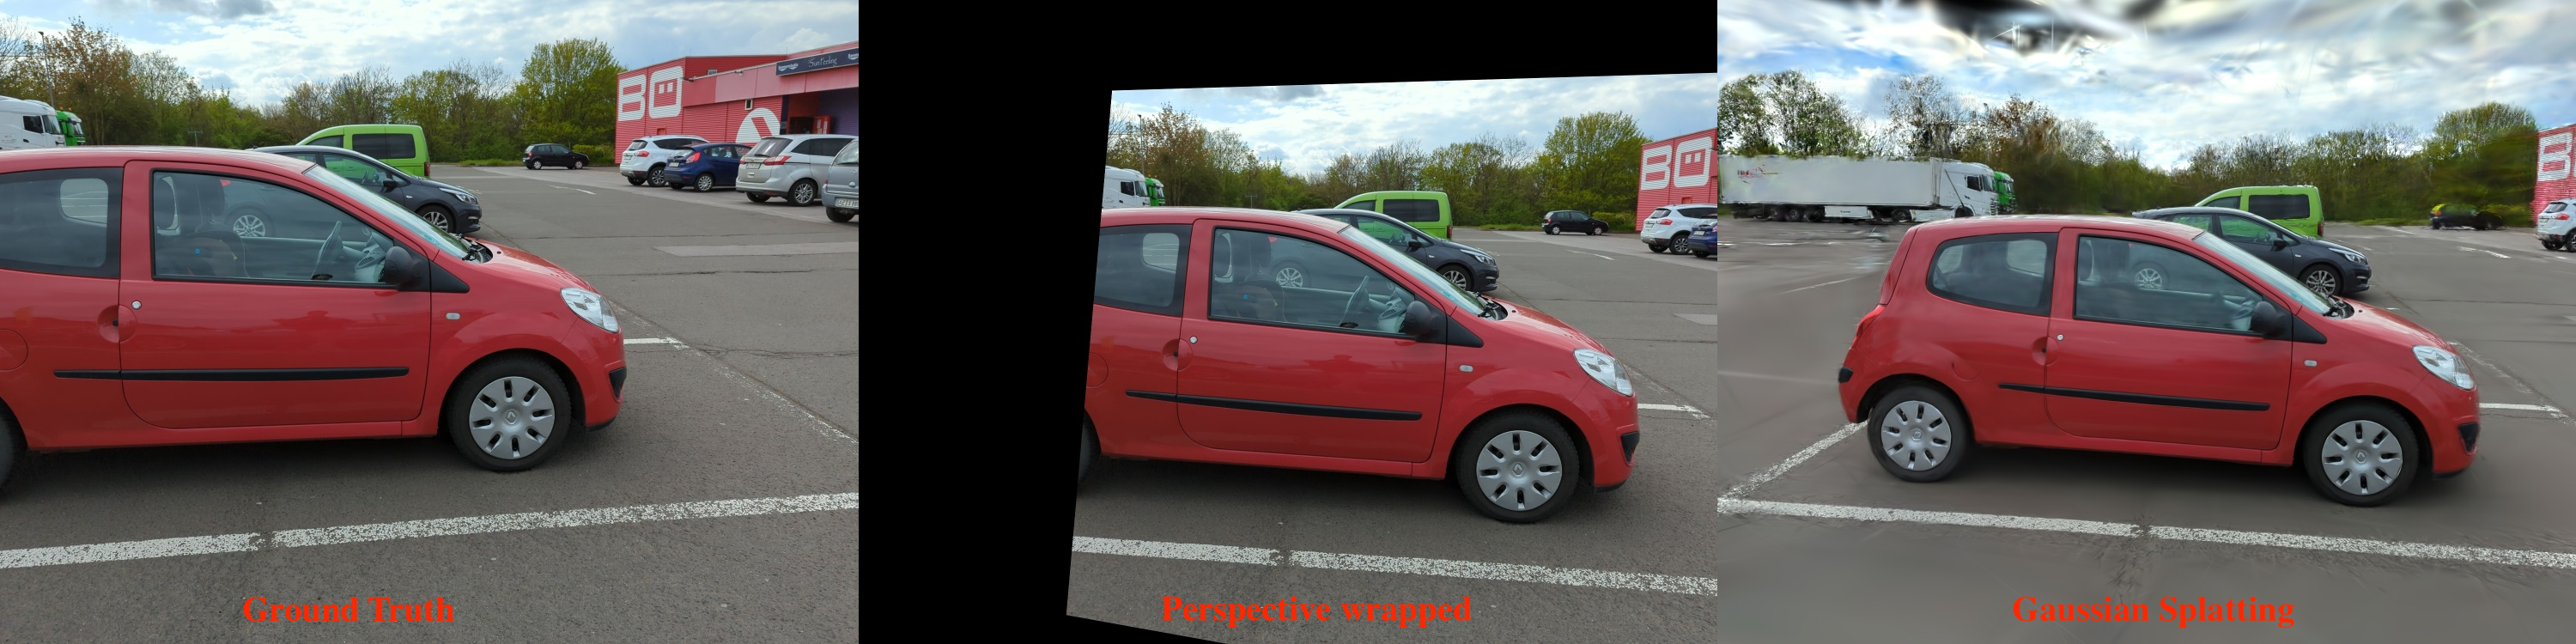
\includegraphics[width=\linewidth]{images/gaussiansplatting/perspective-vs-gs.png}
\caption{\textbf{Perspective transformation and Gaussian Splatting based stabilisation. } Contrary to the homography-based solution, trained GS scene is able to render the whole car. Whereas the car is now properly centred on the view, the perspective-wrapped car is incomplete as the corresponding transformation to apply was too drastic.}
\label{fig:gs-vs-homography-view3}
\end{figure*}

Applying such a transformation to the entire scene, frame by frame, would allow to stabilized the $360^{\circ}$ spin properly. However, as soon as a source view cannot depict the whole car, such an image-based method will fail. 


 
\begin{table}[h!]
  \centering
   \caption{Properties of interest benchmark for $360^{\circ}$ scene stabilization.}
  \begin{tabular}{lcccc}
  \hline
  
    & Complex Reflections & Occlusions & Rendering time & \\
  \hline
  \hline
  Image warp.  & \xmark & \xmark & \cmark \\
  NeRF & \cmark & \cmark & \xmark\\
  GS  & \xmark & \cmark & \cmark \\
  Ours  & \cmark & \cmark & \cmark \\
  \hline
  \label{tab:gs-comp}
  \end{tabular}
\end{table}

We thus leverage in this chapter upon latest advances in neural rendering, and especially on GS-based techniques \citep{kerbl20233d}, to build up a $360^{\circ}$ spin stabilisation pipeline for unbounded scenes. As soon as such a 3D reconstruction system primarily aims to live in a production pipeline for an industrial application, presented methods and experiments extensively focused onto a single scene, that could be one from a car dealership client. As presented on Table \ref{tab:gs-comp}, the pipeline we designed on top of the \ac{GS} one allow us to also tackle reflection and transparent surfaces, without hurting training time or inference performances. 

In summary, we build up an improved 3D reconstruction pipeline based on vanilla \ac{GS} architecture that allows to synthetically render a learn 3D scene at novel viewpoints. Our contributions in this section are three-fold: 
\begin{itemize}
  \item We extend the original sparse SfM point cloud thanks to Silhouette from Motion concept. A 3D visual hull is computed to sample as many points as required to complete the point cloud. 
  \item We direclty leverages upon \citep{malarz2023gaussian} work to make gaussian's opacity view-dependent. Such a modification allows us to better render transparents and reflective surfaces. 
  \item We integrate into our architecture the corrected Adaptative Density Control that PixGS \citep{zhang2024pixelgs} 
    
\end{itemize}

\section{Background: Gaussian Splatting}
A first complete overview of the underlying concepts behind GS is presented in this section. GS leverages on 3D Gaussian primitives to explicitly model the 3D scene. It has a fully differentiable pipeline that can solely be supervised at 2D-image level. Figure \ref{fig:gs-overview} gives few insights regarding how such a pipeline is built. \newline

\begin{figure*}[htb!]
    \center
  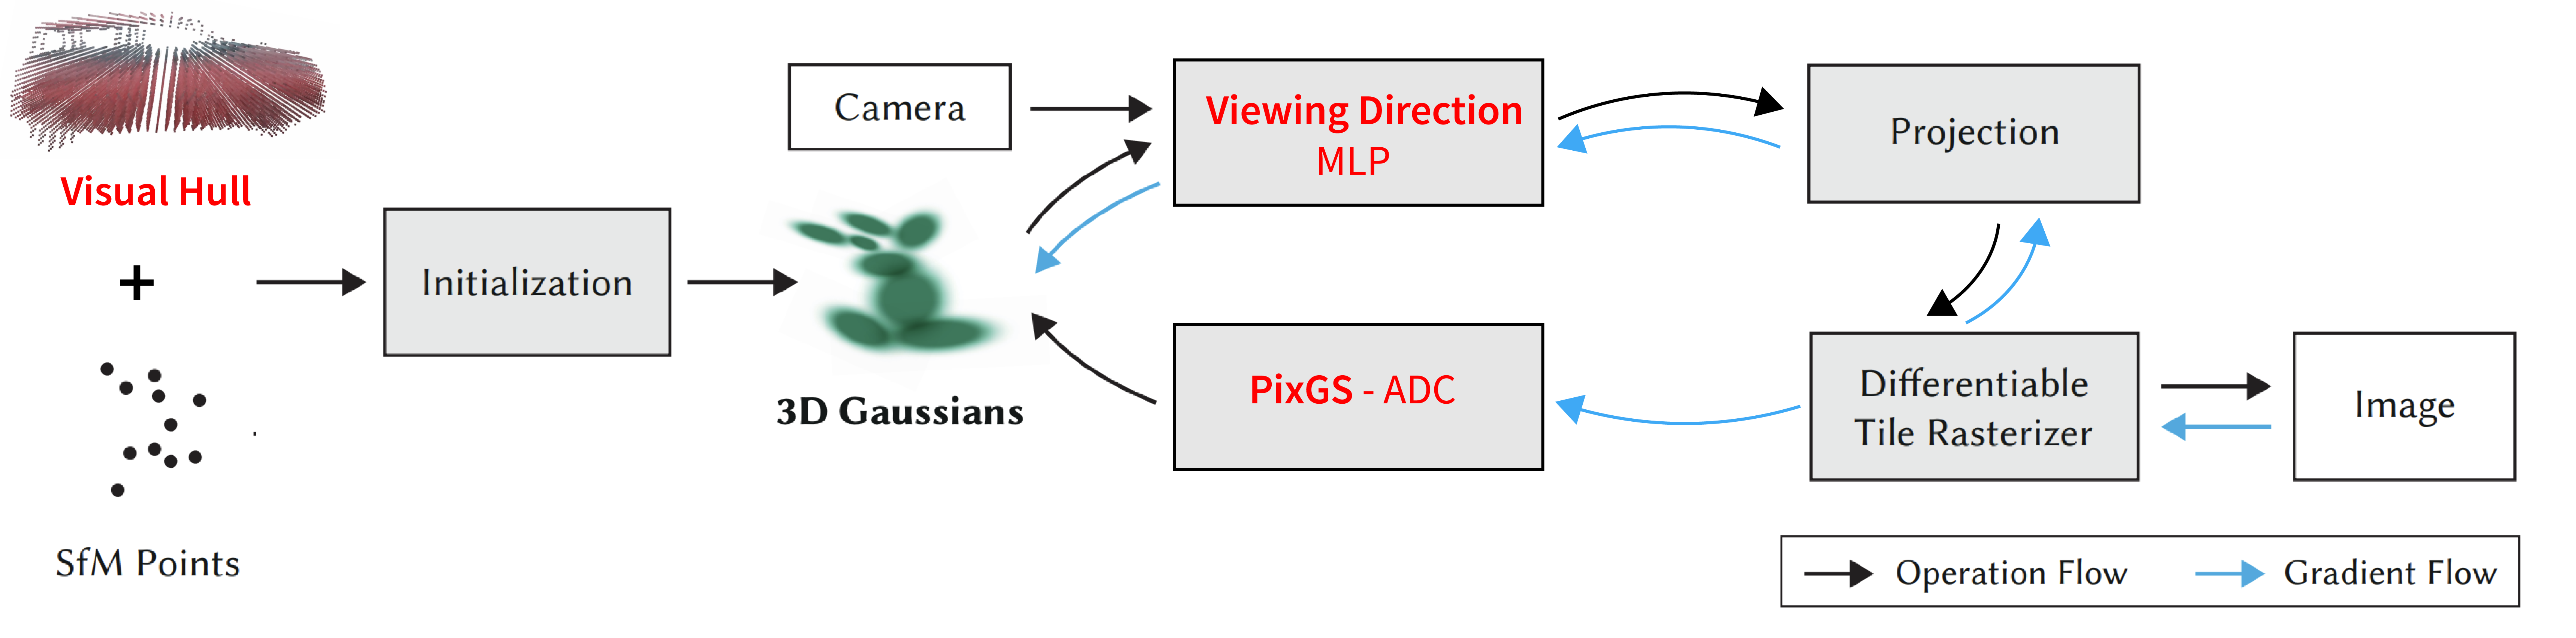
\includegraphics[width=\linewidth]{images/gaussiansplatting/overview_pipeline.png}
  \caption{\textbf{Gaussian Splatting pipeline overview.} Starting from a sparse 3D point cloud, GS is designed on a lightweight and differentiable pipeline that does not involve any deep or shallow neural architectures. \textit{Original illustration comes from the seminal paper}\citep{kerbl20233d} while our modifications are highlighted in \textcolor{red}{red}.}
  \label{fig:gs-overview}
\end{figure*}

We present below the key steps that were defined in the original GS seminal work \citep{kerbl20233d}.


\subsection{Initialization} From a sparse coloured Structure from Motion (SfM)-3D point cloud, referred as $\mathcal{P}\in\mathbb{R}^{N\times(3+3)}$, an associated set of 3D Gaussians $\{\mathcal{G}_{k}|k=1,...,K\}$ is build. Each primitive $\mathcal{G}_{k} $ has therefore an attached set of learnable attributes, defined in the Table \ref{tab:gauss-param}. 


\begin{table}[h!]
  \centering
   \caption{Per gaussian $\mathcal{G}_{k} $  parameters that need to be optimized.}
  \begin{tabular}{lcc}
  \hline
  Parameter  & Size & Note \\
  \hline
  Position (mean)  $\mu^{(k)}_{3D}$ & 3 & 3D vector $(x, y, z)$ \\
  3D Covariance $\Sigma^{(k)}_{3D}$ & 7 & 3D vector $(x, y, z)$ + scalar + 3D vector  $(i, j, k)$\\
  Opacity  $o^{(k)}$ & 1 & scalar \\
  SH coefficients  $c^{(k)}$ & 48 & 4 bands of SH; $(1+3+5+7)\times3$ \\
  \hline
  Total (per Gaussian)  & 59 & \\
  \hline
  \end{tabular}
 
  \label{tab:gauss-param}
\end{table}

While mean, color and opacity can be optimised without any constraints with gradient-descent based algorithm, $\Sigma^{(k)}_{3D}$ has to remain semi-definite positive \footnote{\textit{i.e} $ \forall a \in \mathbb{R}^{3}: a^{T}\Sigma^{(k)}_{3D}a \geq 0$} during training to represent a meaningful 3D coviance matrix. As holding this constraint during the optimization would be to complex, $\Sigma^{(k)}_{3D}$ is factorized (as an eigendecomposition) in the world coordinate system via with a rotation matrix $O_{k}$ (analytically expressed with 4 quaternions) and a scaling vector $s_{k}$: 

\begin{equation}
    \Sigma^{(k)}_{3D} = O_{k}s_{k}s_{k}^{T}O_{k}^{T}
\end{equation}
As any matrix expressed with $A^{T}A$ is always semi-definite positive, $\Sigma^{(k)}_{3D}$ is now properly constrained. 

Considering any point \textit{p} in the world 3D space, the geometry of a primitive $\mathcal{G}_{k}$ has an influence over \textit{p} that can be expressed through: 

\begin{equation}
  \mathcal{G}_{k}(p) = \exp \left(-\frac{1}{2}(p-\mu^{(k)}_{3D})^{T}(\Sigma^{(k)}_{3D})^{-1}(p-\mu^{(k)}_{3D})\right)
\end{equation}

\subsection{3D Gaussian projection} The 3D Gaussian parameters are optimised during training phase by only leveraging on an image-based supervision signal. The 3D ellipsoids must thus be render on 2D image plane in a differentiable manner and a corresponding 2D mean and covariance need to be derived from $\mu^{(k)}_{3D}$ and $\Sigma^{(k)}_{3D}$ for each primitive using EWA splatting \citep{zwicker2001ewa}. 

Given any viewpoint we want to render, let's denote corresponding world-to-camera extrinsic matrix $W=[R|t]$ and the intrinsic $K$. The gaussian center $\mu^{(k)}_{3D}$ is easily projected in 2D through the perspective projection: 

\begin{equation}
  \begin{bmatrix}
    u \\
    v \\
    z
  \end{bmatrix} = KW\mu^{(k)}_{3D} = K(R\mu^{(k)}_{3D}+t) = K \mu^{(k)}_{cc}
\end{equation}
where $\mu^{(k)}_{cc}$ refers to 3D location expressed in the camera coordinate system. Finally, the 2D mean $\mu^{(k)}_{2D} = \begin{bmatrix}
  u/z \\
  v/z
\end{bmatrix}$ can be  thus expressed in the pixel coordinate system as:
\begin{equation}
  \mu^{(k)}_{2D} = K(W\mu^{(k)}/(W\mu^{(k)}_{z})) = K(\mu^{(k)}_{cc}/(\mu^{(k)}_{cc,z}))
\end{equation}
We finally denotes by $\mu^{(k)}_{ncd}$ the 2D mean expressed in the NDC coordinate system from $\mu^{(k)}_{2D}$. 

Regarding the 3D covariance, $\Sigma^{(k)}$ is expressed in the camera coordinate system through: 

\begin{equation}
  \Sigma^{(k)}_{cc}= R\Sigma^{(k)}_{3D}R^{T}
  \label{eq:gs-3dcov-transfrom}
\end{equation}

and in image/ray space as:
\begin{equation}
  \Sigma^{(k)}_{ic}= J_{k}\Sigma^{(k)}_{cc}J_{k}^{T}
  \label{eq:gs-3d2dcov}
\end{equation}

where $J = \partial \mu^{(k)}_{2D} / \partial \mu^{(k)}_{3D}$ is the Jacobian of the mean projection formula (\textit{i.e} the affine approximation of the 3D-2D projection).


As explained in \citep{zwicker2001ewa}, one can drop the thrid row and column of  $ \Sigma^{(k)}_{ic}$ to get a 2D covariance matrix, named $\Sigma^{(k)}_{2D}$. Applying a projective transformation to any 3D gaussian primitive $\mathcal{G}_{k}$ lead to another scaled 2D gaussian primitive, termed $g_{k}$: 

\begin{equation}
  g_{k}(x) = \exp(-\frac{1}{2}(x-\mu^{(k)}_{2D})^{T}(\Sigma^{(k)}_{2D})^{-1}(p-\mu^{(k)}_{2D}))
\end{equation}

3DGS seminal work \citep{kerbl20233d} finally performs alpha blending to render a color $\hat{c}(x)$ through: 

\begin{equation}
\label{eq:gs-alpha-blending}
  \hat{c}(x) = \sum_{k=1}^{K}c_{k}\alpha_{k}\prod_{j=1}^{k-1}(1-\alpha_{j})
\end{equation}

\begin{equation}
\label{eq:gs-alpha-def}
  \alpha_{k} = o_{k}g_{k}(x)
\end{equation}

where primitive’s depth order are sorted from 1 to K. \newline

\subsection{ADC} 
As the original SfM point cloud can be extremely sparse, authors from \citep{kerbl20233d} implement both a densification and pruning strategy during training. 

The pruning is quite simple yet effective: any 3D gaussian that has an opacity $\alpha$ below a fixed threshold $\epsilon_{\alpha}$ during training is removed from $\mathcal{G}$. 

The densification strategy requires to both address under-reconstructed areas (where an insufficient number of gaussians are present) and over-reconstructed areas (where gaussians are too large) of the scene. Small gaussians are thus cloned in those under-reconstructed areas whereas large ones are splited into two new gaussians by leveraging on view-space positional gradients, expressed for each gaussian primitive $\mathcal{G}_{k}$ as : 

\begin{equation}
   \nabla_{\mu_{k}}L= ||\frac{\partial L_{\pi}}{\partial \mu_{k}^{\pi}}|| = \sqrt{\left(\frac{\partial L_{\pi}}{\partial \mu_{ndc,x}^{k,\pi}}\right)^{2} + \left(\frac{\partial L_{\pi}}{\partial \mu_{ndc,y}^{k,\pi}}\right)^{2}}
\end{equation}

where $L_{\pi}$ denotes the loss under viewpoint $\pi$. Such a gradient magnitude is tracked and averaged over all the rendered views $\pi \in \Pi$ during 100 iterations. When: 

\begin{equation}
\frac{\sum \limits_{\pi \in \Pi} ||\frac{\partial L_{\pi}}{\partial \mu_{k}^{\pi}}||}{\sum \limits_{\pi \in \Pi} 1} > \tau_{pos}
\label{eq:adc-original}
\end{equation}
holds for gaussian primitive $\mathcal{G}_{k}$, the latter is either splited or cloned depending on its size. Largest eigenvalue of $\Sigma_{k}$ is used to status on $\mathcal{G}_{k}$ size: if such an eigenvalue is above another fixed user defined threshold, primitive is splited, cloned otherwise. \newline

\subsection{Differentiable rasterizer} As soon as the supervisory signal is 2-dimensional, one can leverage onto a differentiable rasterizer to made such pipeline end-to-end trainable. We provide the key steps of such a tile-based rasterizer: 

\begin{enumerate}
    \item Image screen is divided into $16\times 16$ 
\end{enumerate}

\subsection{Training} 
Gaussians parameters are learned during training through the vanilla stochastic gradient descent optimization procedure. The corresponding loss function is expressed through: 
\begin{equation}
    \mathcal{L} = (1-\lambda)\mathcal{L}_{1}(I_{GT},\hat{I}) + \lambda \mathcal{L}_{D-SSIM}(I_{GT},\hat{I})
\end{equation}

\section{Our 3D GS-based pipeline}
We now extensively present in this section the 3D gaussian splatting system we designed for our $360^{\circ}$ spin rendering stabilization problem. We build up our system on top of three distinct strategies, that all consistently improve the overall pipeline. 

\subsection{Viewing Direction}
First bloc we get into consideration on top of the existing GS vanilla framework come from ViewingDirection-GS (VDGS) \citep{malarz2023gaussian}. Core authors idea is to some extend mix concepts from both NeRF and GS to get the most of both framework, as depicted on Figure \ref{fig:gs-nerf}. 

\begin{figure}[htpb!]
  \centering
  \begin{subfigure}[b]{0.31\linewidth}
    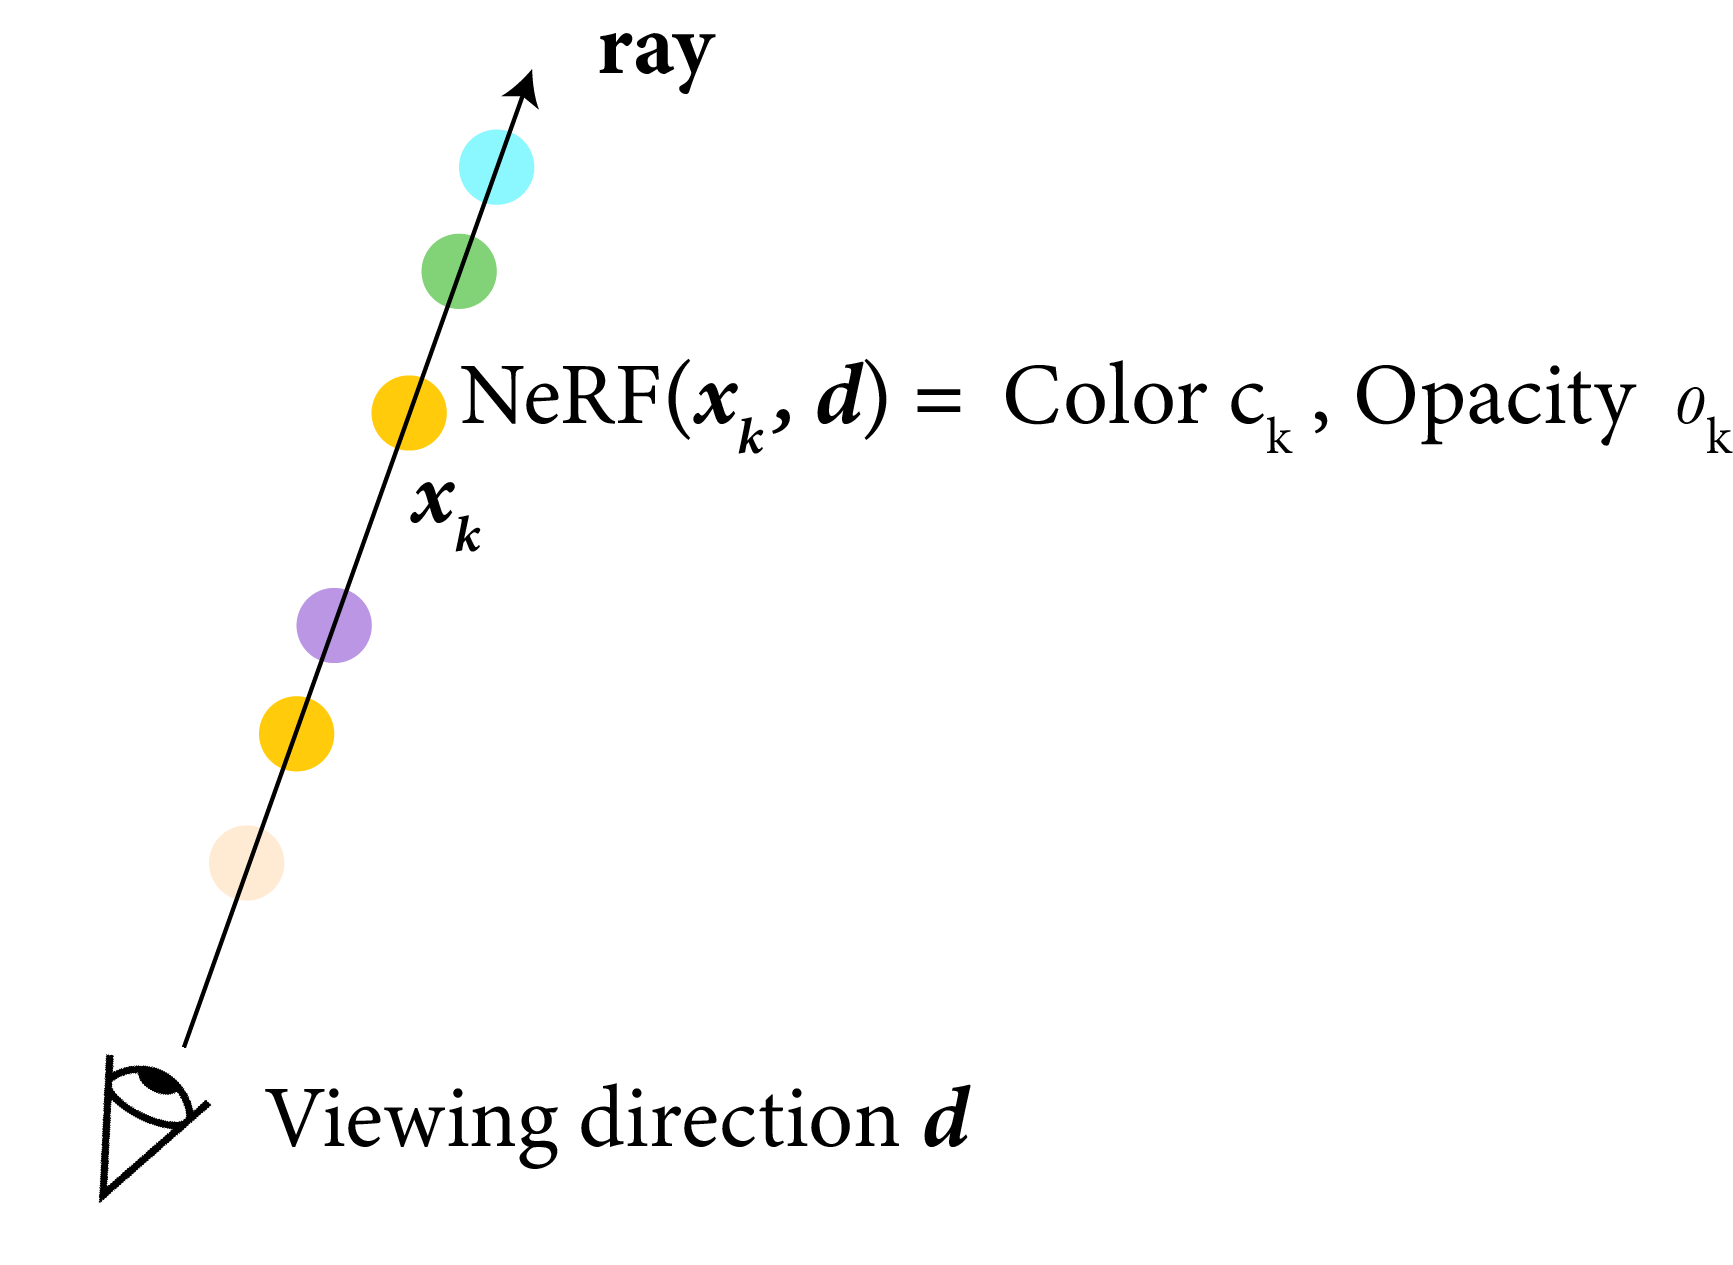
\includegraphics[width=\linewidth]{images/gaussiansplatting/nerf.png}
    \caption{\textbf{NeRF-based}}
    \label{fig:nerf-ray}
  \end{subfigure}
  \quad % Space between the figures
  \begin{subfigure}[b]{0.31\linewidth}
    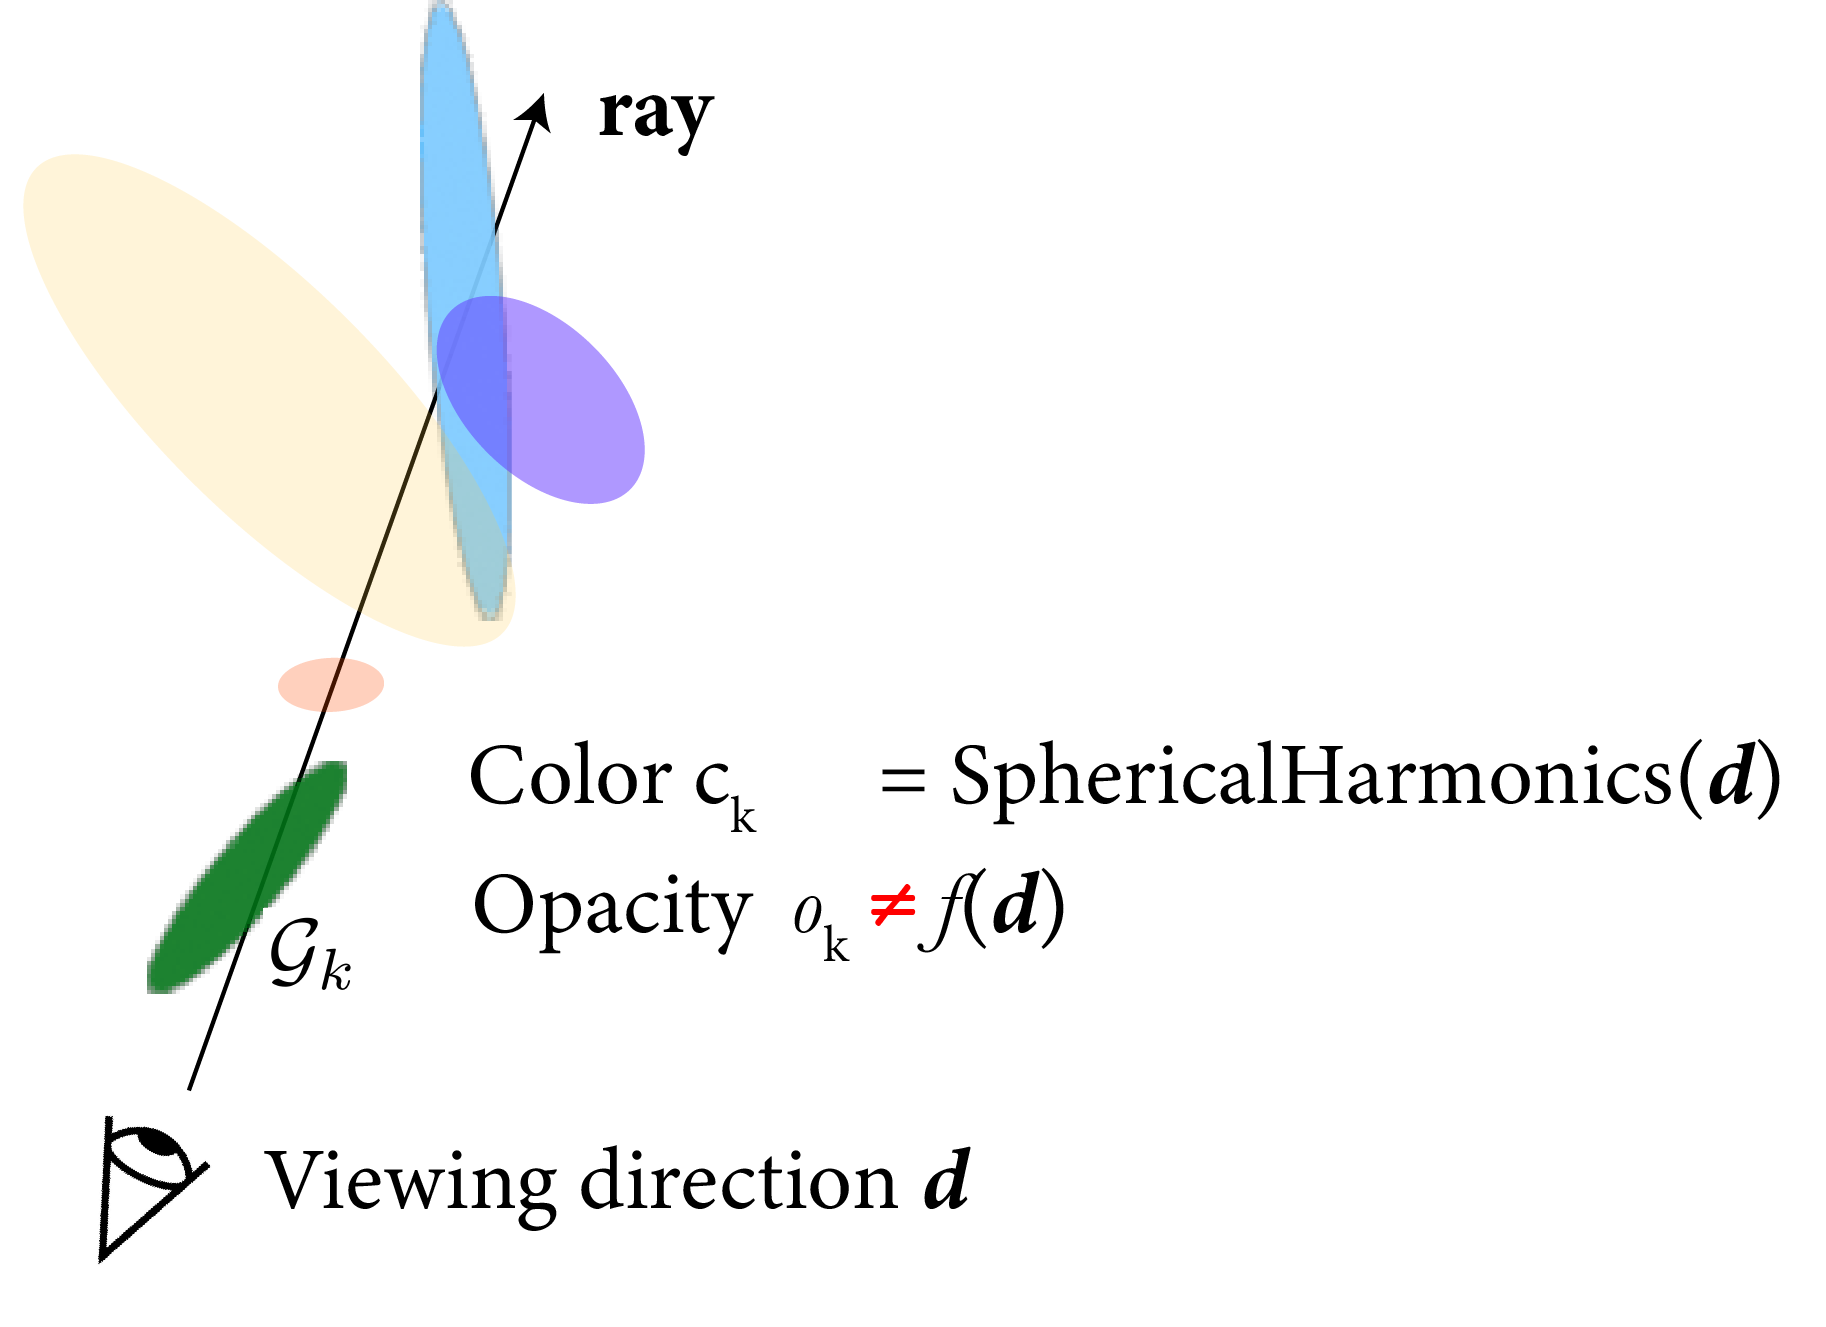
\includegraphics[width=\linewidth]{images/gaussiansplatting/gs_vanilla.png}
    \caption{\textbf{GS-based}}
    \label{fig:gs-ray}
  \end{subfigure}
  \quad % Space between the figures
  \begin{subfigure}[b]{0.31\linewidth}
    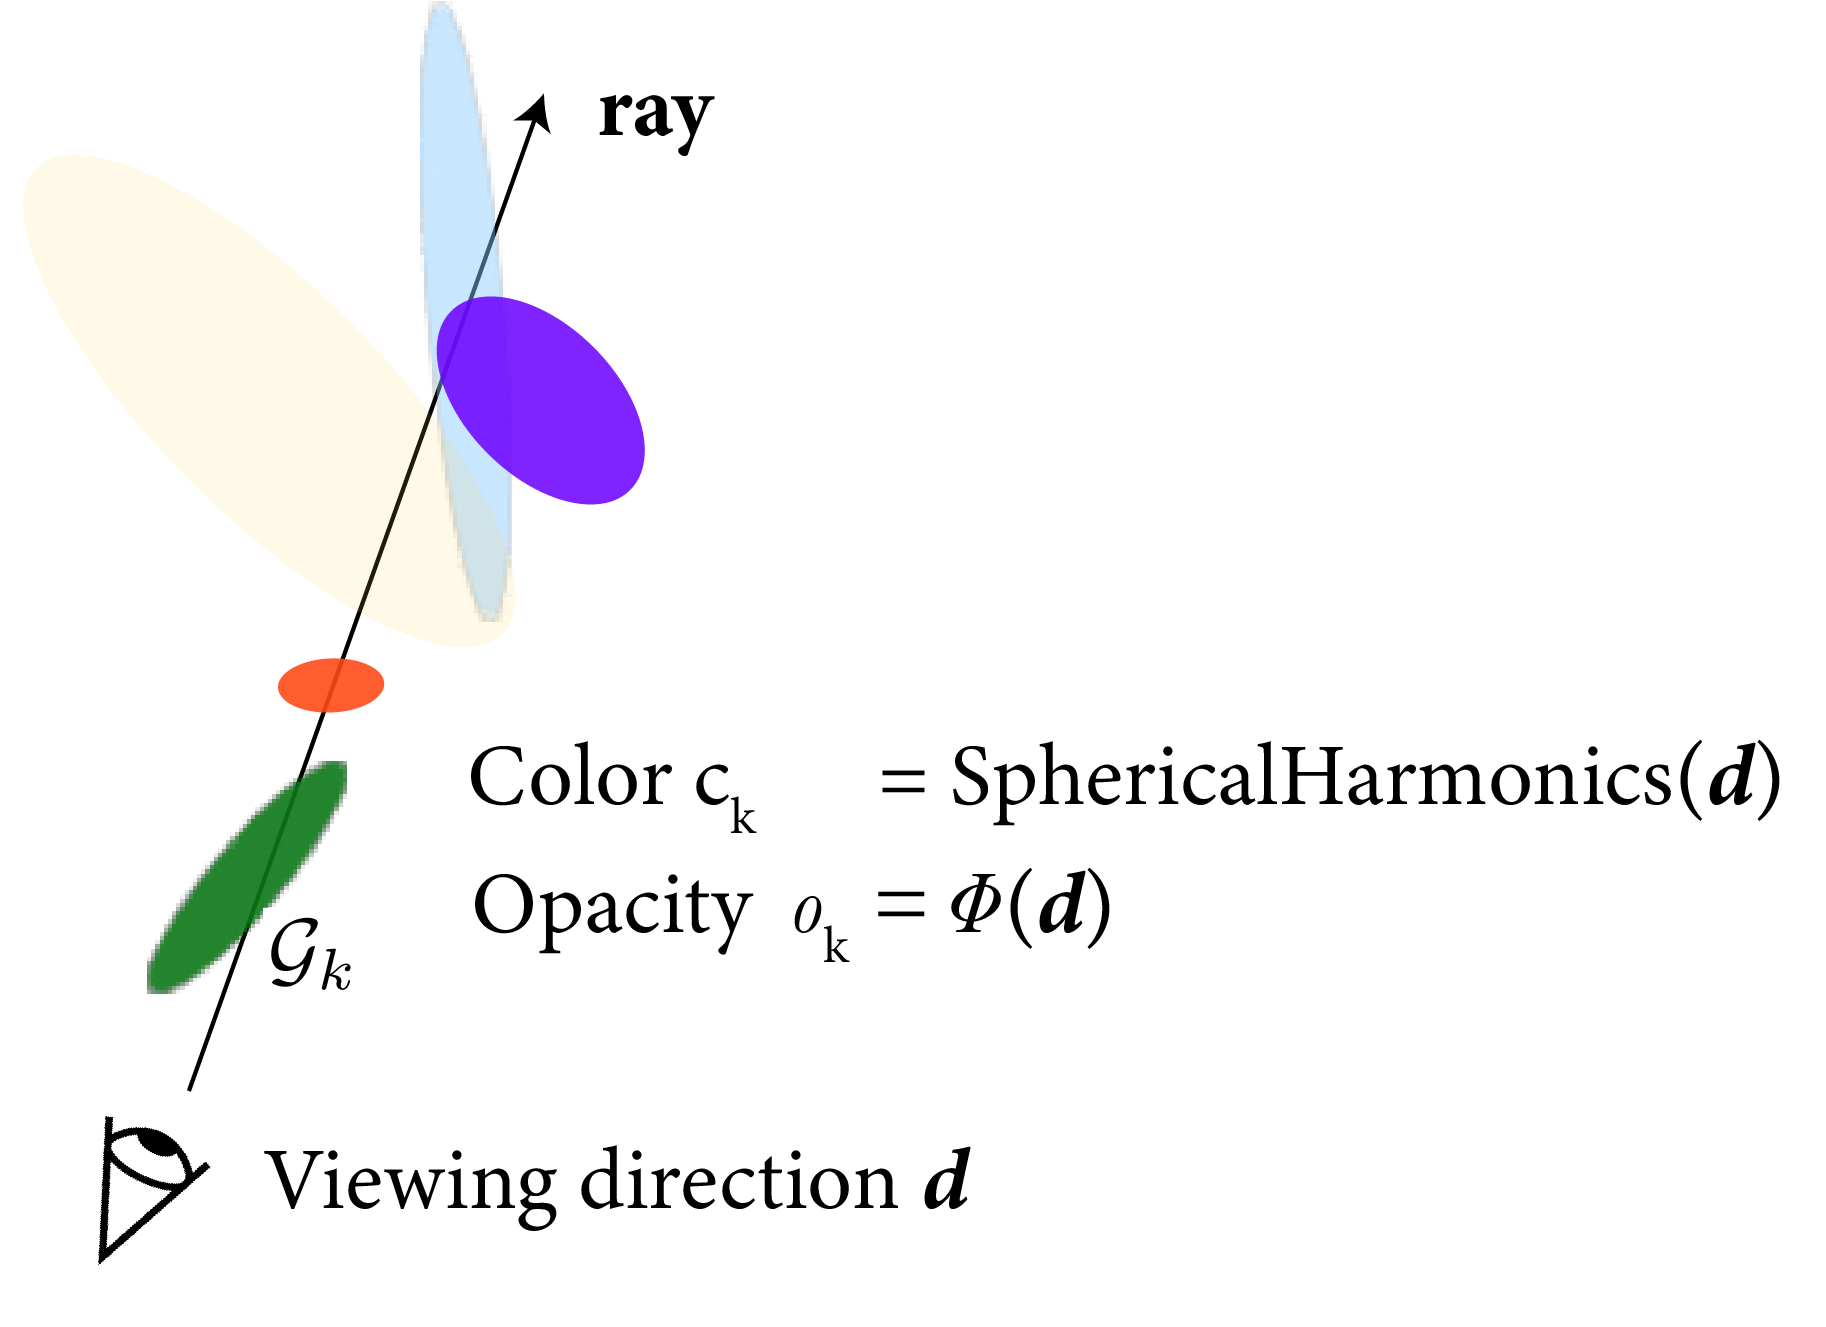
\includegraphics[width=\linewidth]{images/gaussiansplatting/gs.png}
    \caption{\textbf{Ours}}
    \label{fig:gs-ray}
  \end{subfigure}
  \caption{\textbf{Conceptual difference between NeRF and GS.} Neural radiance fields output color and opacity as a function of the viewing direction. GS original code solely encodes view dependency through the spherical harmonics \textit{sh} basis. Our modification allows to also output the opacity value of each primitive as a function of \textbf{d}. }
  \label{fig:gs-nerf}
\end{figure}

The trained GS scene remains expressed as a 3D gaussians cloud but authors introduced an additional Multi-Layer Perceptron (MLP) that is going to output a corrective update on each gaussian opacity. 

Indeed, each primitive has an opacity property but the latter does not depend on the viewing direction \textbf{d} we looking at during rasterization. Introducing such an MLP, termed $\Phi$ therefore aims to alter gaussian transparency in function of this viewing direction: 

\begin{equation}
\Delta o_{k} = \Phi(\Sigma_{k},c_{k},\textbf{d}) 
\end{equation}

so that the final corrected opacity $o_{k}^{corr.}$ is expressed as: 

\begin{equation}
o_{k}^{corr.} = \Delta o_{k}(\textbf{d}) \times o_{k} 
\end{equation}

This novel view-dependency opacity allow the pipeline we build specifically for car scenes to better handle surface light reflections as well as transparent regions on windows.

The alpha-blending equation, introduced in equation (\ref{eq:gs-alpha-blending}) remains unchanged to get the final rendered pixel color.

Such a lightweight MLP $\Phi$ thus highly improve the light reflections and windows transparency issue we often encounter in our car scenes. In-depth quantitative figures as well as visual insights on the usefulness of such an opacity view dependency are presented in detail in section \ref{sec:exp}. 

\subsection{Visual Hull}

We present in this section a complementary way to get another initial point cloud $\mathcal{P}$ to start GS scene training. 


\begin{figure*}[htbp!]
    \center
  \includegraphics[width=\linewidth]{images/gaussiansplatting/image_sift.png}
  \caption{\textbf{SIFT correspondence between 2 closed views} SIFT keypoints detection and matching from COLMAP struggle a lot on such a reflective scene. Only a very limited number of key-points has been properly matched (in bold).}
  \label{fig:sift-colmap}
\end{figure*}

Most of the SIFT keypoints COLMAP-SfM algorithm relies on do not lie on the car surface, as reflections are extremely hard to handle. Such a claim can be seen on Figure \ref{fig:sift-colmap}. Only a very limited number of SIFT points have been properly matched each other on the two views. Such a poor detection and matching performance led to a 
final point cloud that is extremely sparse: $\mathcal{P}$ has only roughly 4K points and most of them do not live on the car surface, as seen on Figure \ref{fig:sfm-colmap-pc}. 

\begin{figure*}[htbp!]
    \center
  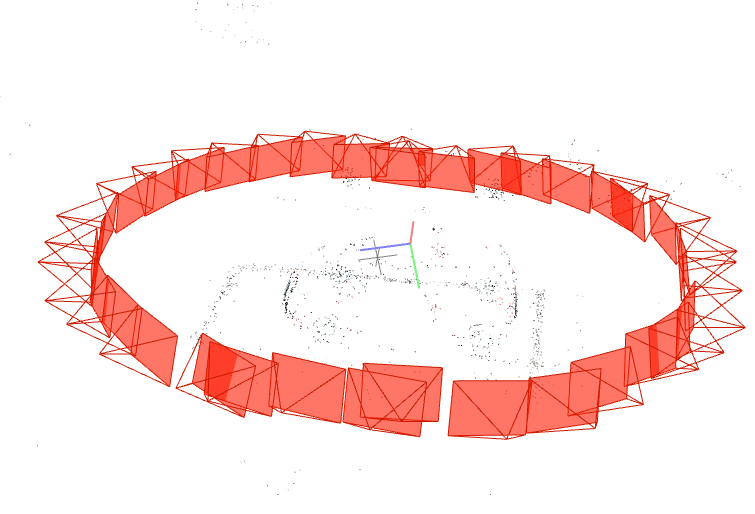
\includegraphics[width=.8\linewidth]{images/gaussiansplatting/colmap_sparsePC.png}
  \caption{\textbf{Final SfM point cloud with predicted camera poses} Wheareas 36 views were involved in the SfM-point cloud construction, only few points lie on the car surface we aim to reconstruct in 3D.}
  \label{fig:sfm-colmap-pc}
\end{figure*}


\begin{figure}[htpb!]
  \centering
  \begin{subfigure}[b]{0.48\linewidth}
    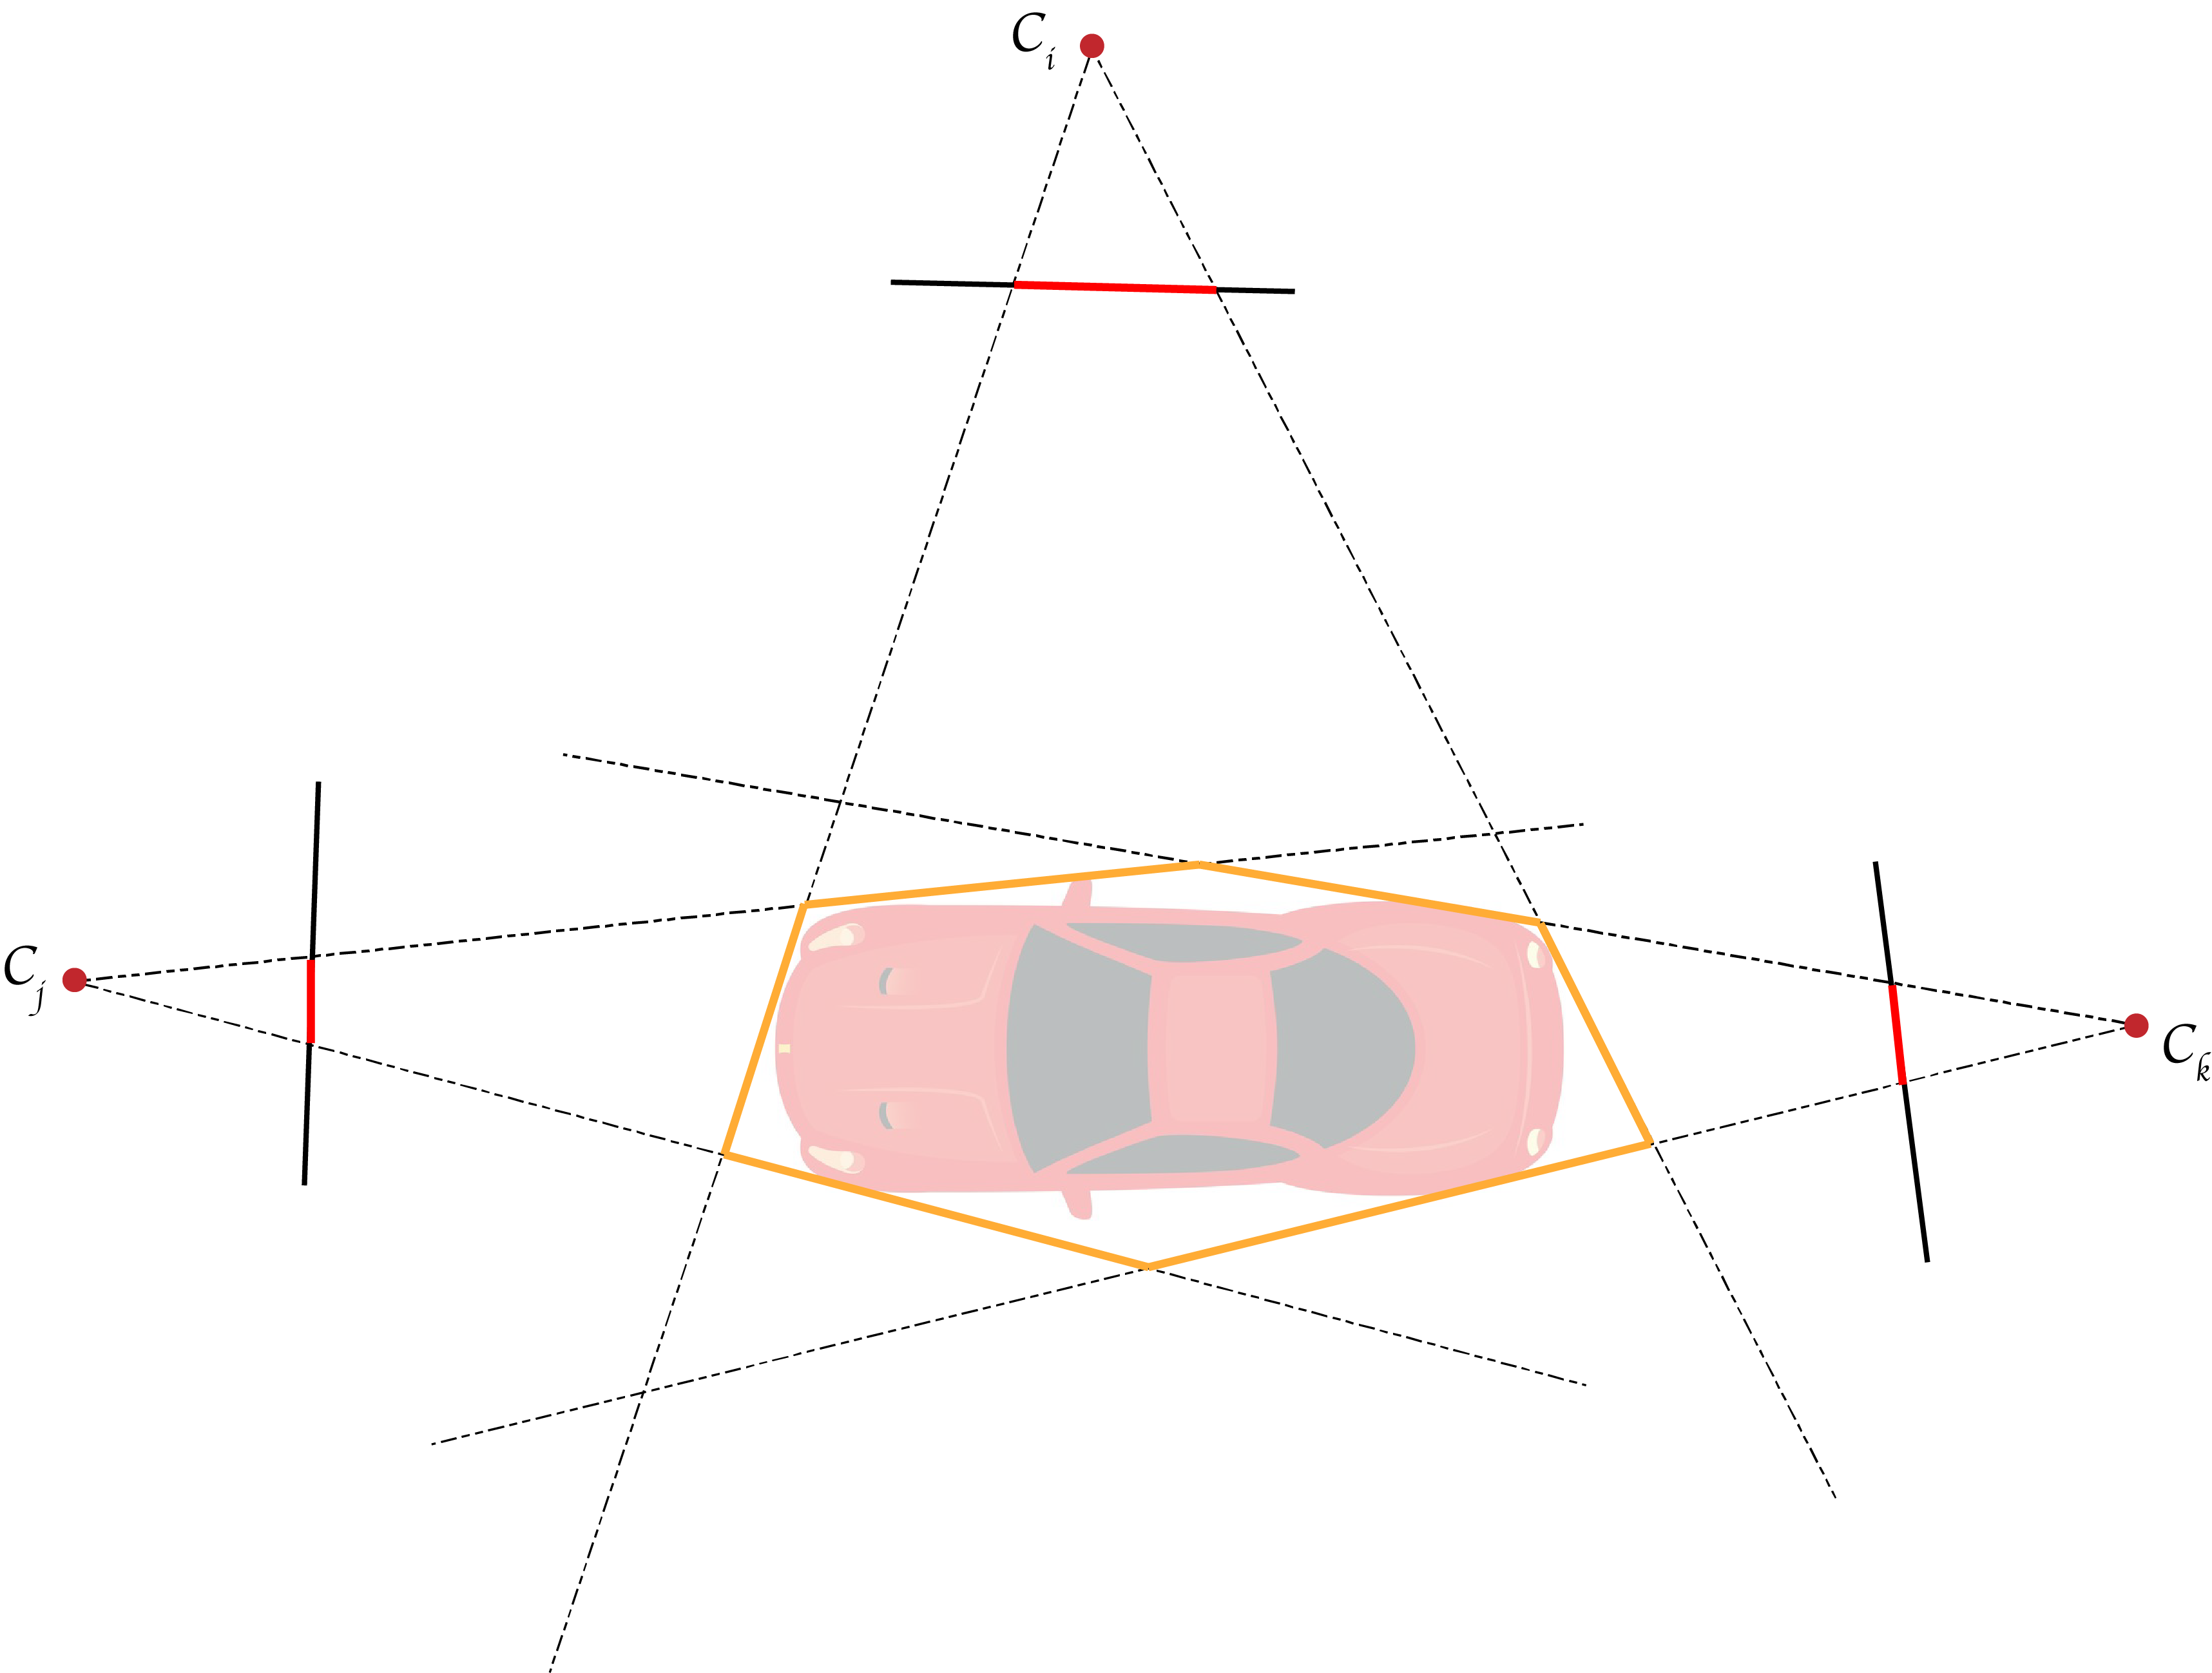
\includegraphics[width=\linewidth]{images/gaussiansplatting/visualhull-idea.png}
    \caption{\textbf{Overview idea}}
    \label{fig:gs-vh-concept}
  \end{subfigure}
  \quad % Space between the figures
  \begin{subfigure}[b]{0.48\linewidth}
    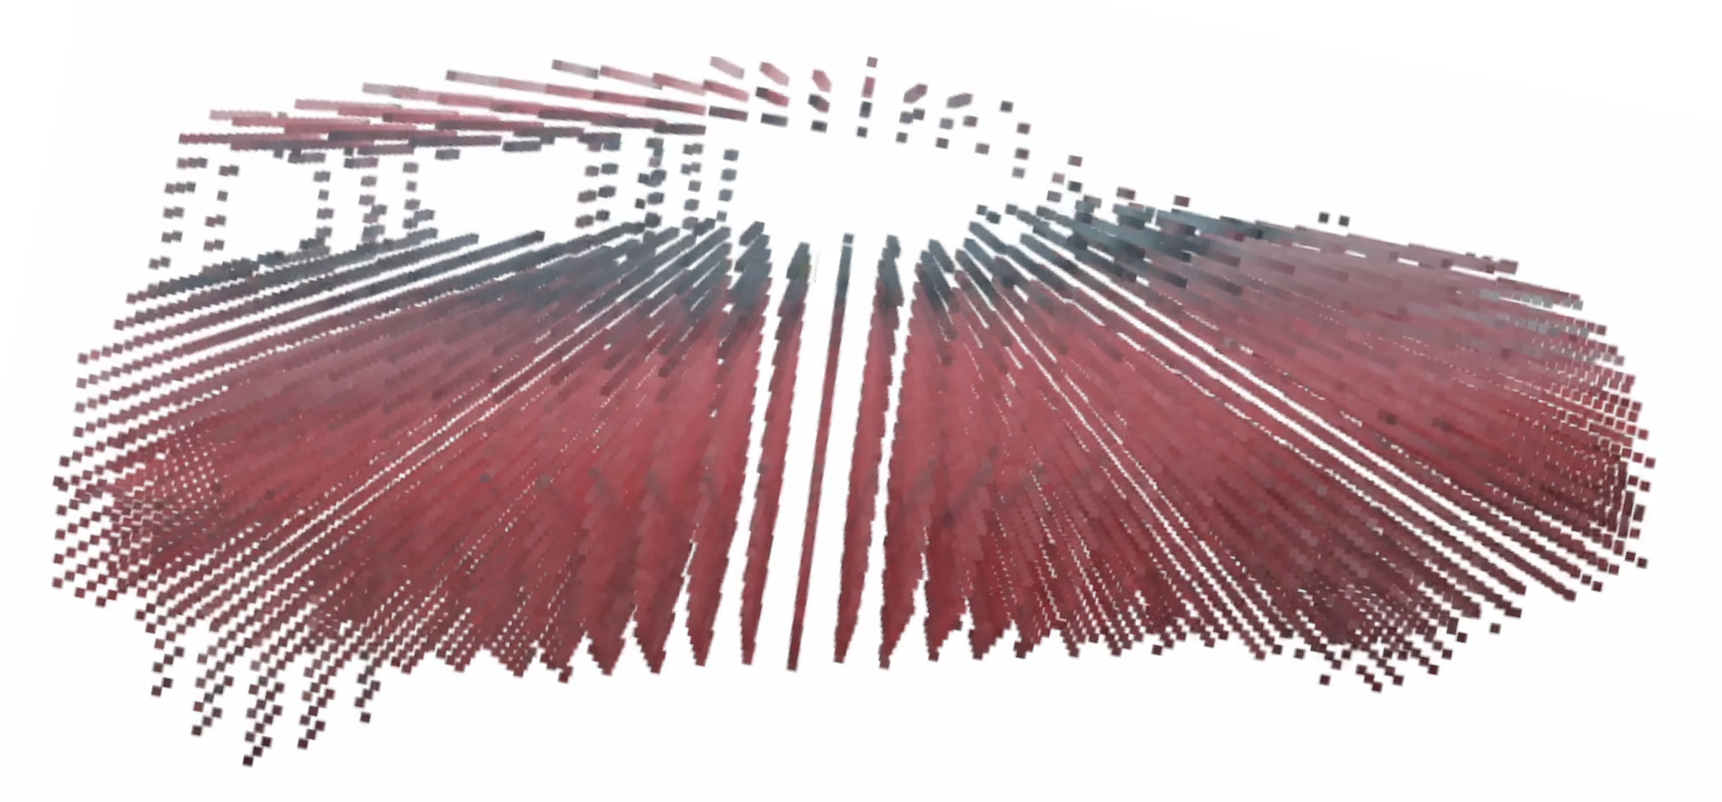
\includegraphics[width=\linewidth]{images/gaussiansplatting/visualhull-res.png}
    \caption{\textbf{Resulting hull}}
    \label{fig:gs-vh-result}
  \end{subfigure}
  \caption{\textbf{Visual hull concept.} A visual hull is here built as the intersection of three 3D bounding cones from the silhouette masks. Such hull is almost convex in case of our car scenario. One can  sample 3D points within the visual hull to build a new dense point cloud.}
  \label{fig:gs-homography-view3}
\end{figure}


We consider a novel point cloud method initialisation by leveraging upon a visual hull, a silhouette-from-motion \citep{baumgart1974geometric} based-concept. It only requires to get the posed images $\{I_{i},\pi_{i}\}_{i=1}^{N}$ and the corresponding binary silhouette masks $\mathcal{S}$. The Figure \ref{fig:gs-vh-concept} allows to grasp the visual hull concept. 

We present on Algorithm \ref{alg:gs-vh} the pseudo code that allow to generate such a visual hull (VisHull) point cloud. 

\begin{algorithm}[htpb!]
  \caption{Visual hull contruction}\label{alg:gs-vh}
  \SetKwInOut{Input}{input}
  \SetKwInOut{Output}{output}
  \SetKwInOut{Parameter}{parameter}
  \Input{Images $\mathcal{I}$, Silhouette mask $\mathcal{S}$}
  \Parameter{Intrinsic and extrinsic camera parameters $\pi=K[R|t]$}
  \Output{Visual hull-based point cloud $\mathcal{P}_{VH}$ } 
  \medskip
  \KwResult{$\mathcal{P}_{VH}$ can be densely sampled}
  \medskip
  $bbox \gets \mathbf{build3DBB}()$ \tcp*[l]{Create a vanilla 3D bounding boxe}
  $P_{3D} \gets \mathbf{sampleDensely}(bbox)$\hspace{.4cm}\textcolor{gray!80}{\# 
    [$N_{pts}$,3]} \tcp*[l]{Sample points in the BB}

   $P_{2D} \gets \mathbf{project}(P_{3D},\pi)$ \hspace{.4cm}\textcolor{gray!80}{\# 
    [$N_{pts}$,2]} \tcp*[l]{Reproject on image plane }
    
    $idx_{valid} \gets \mathbf{keepValidPoints}(P_{2D},\mathcal{M})$ \hspace{.4cm}\textcolor{gray!80}{\# 
    [$N_{pts}$,1]} \tcp*[l]{Boolean. 1 if valid, 0 otherwise}

    $P_{3D}^{(refined)} \gets P_{3D}[idx_{valid}]$ 

    $P_{VH} \gets \mathbf{setRGBcolor}(P_{3D}^{(refined)},P_{2D},idx_{valid},\mathcal{I})$ \tcp*[l]{Set RGB color to the point cloud through bilinear interpolation}
\end{algorithm}

\subsection{PixGS ADC}
\label{gs:pixgs-adc}
Our latest improvement of the vanilla GS framework is directly link to the way gaussians are splited and cloned during the \ac{ADC} procedure. We extensively leverage upon PixGS \citep{zhang2024pixelgs} to change update the densification formulation.  

Original \ac{ADC} strategy has several inner limitations in its current form: 
\begin{itemize}
    \item Per-pixel gradient involved in $\frac{\partial L_{\pi}}{\partial \mu^{k,\pi}_{ndc,x}}$ and $\frac{\partial L_{\pi}}{\partial \mu^{k,\pi}_{ndc,y}}$  have different directions. It lead to some gradient collision, were magnitude of $\frac{\partial L_{\pi}}{\partial \mu_{k}^{\pi}}$ does not reach densification threshold while it should. 
    \item Properly setting the two threshold involved in the densification process is not intuitive: optimal threshold values might vary from a scene to another one. 
    \item There is no explicit control regarding the total number of gaussians a scene can reach, leading to potential \textit{OOM} issues.
\end{itemize}

Sparse point cloud areas lead to large ellipsoids gaussian during initialisation as soon as axes length are set considering the nearest neighboring points. Large gaussians are thus involved in loss computation from too many viewpoints. However, summing over a large number of viewpoint and  number of pixels gradients that have different direction could lower down the total magnitude \ac{ADC} is tracking for densification. Such a behaviour is illustrated on Figure \ref{fig:adc-limitation}



\begin{figure*}[htbp!]
    \center
  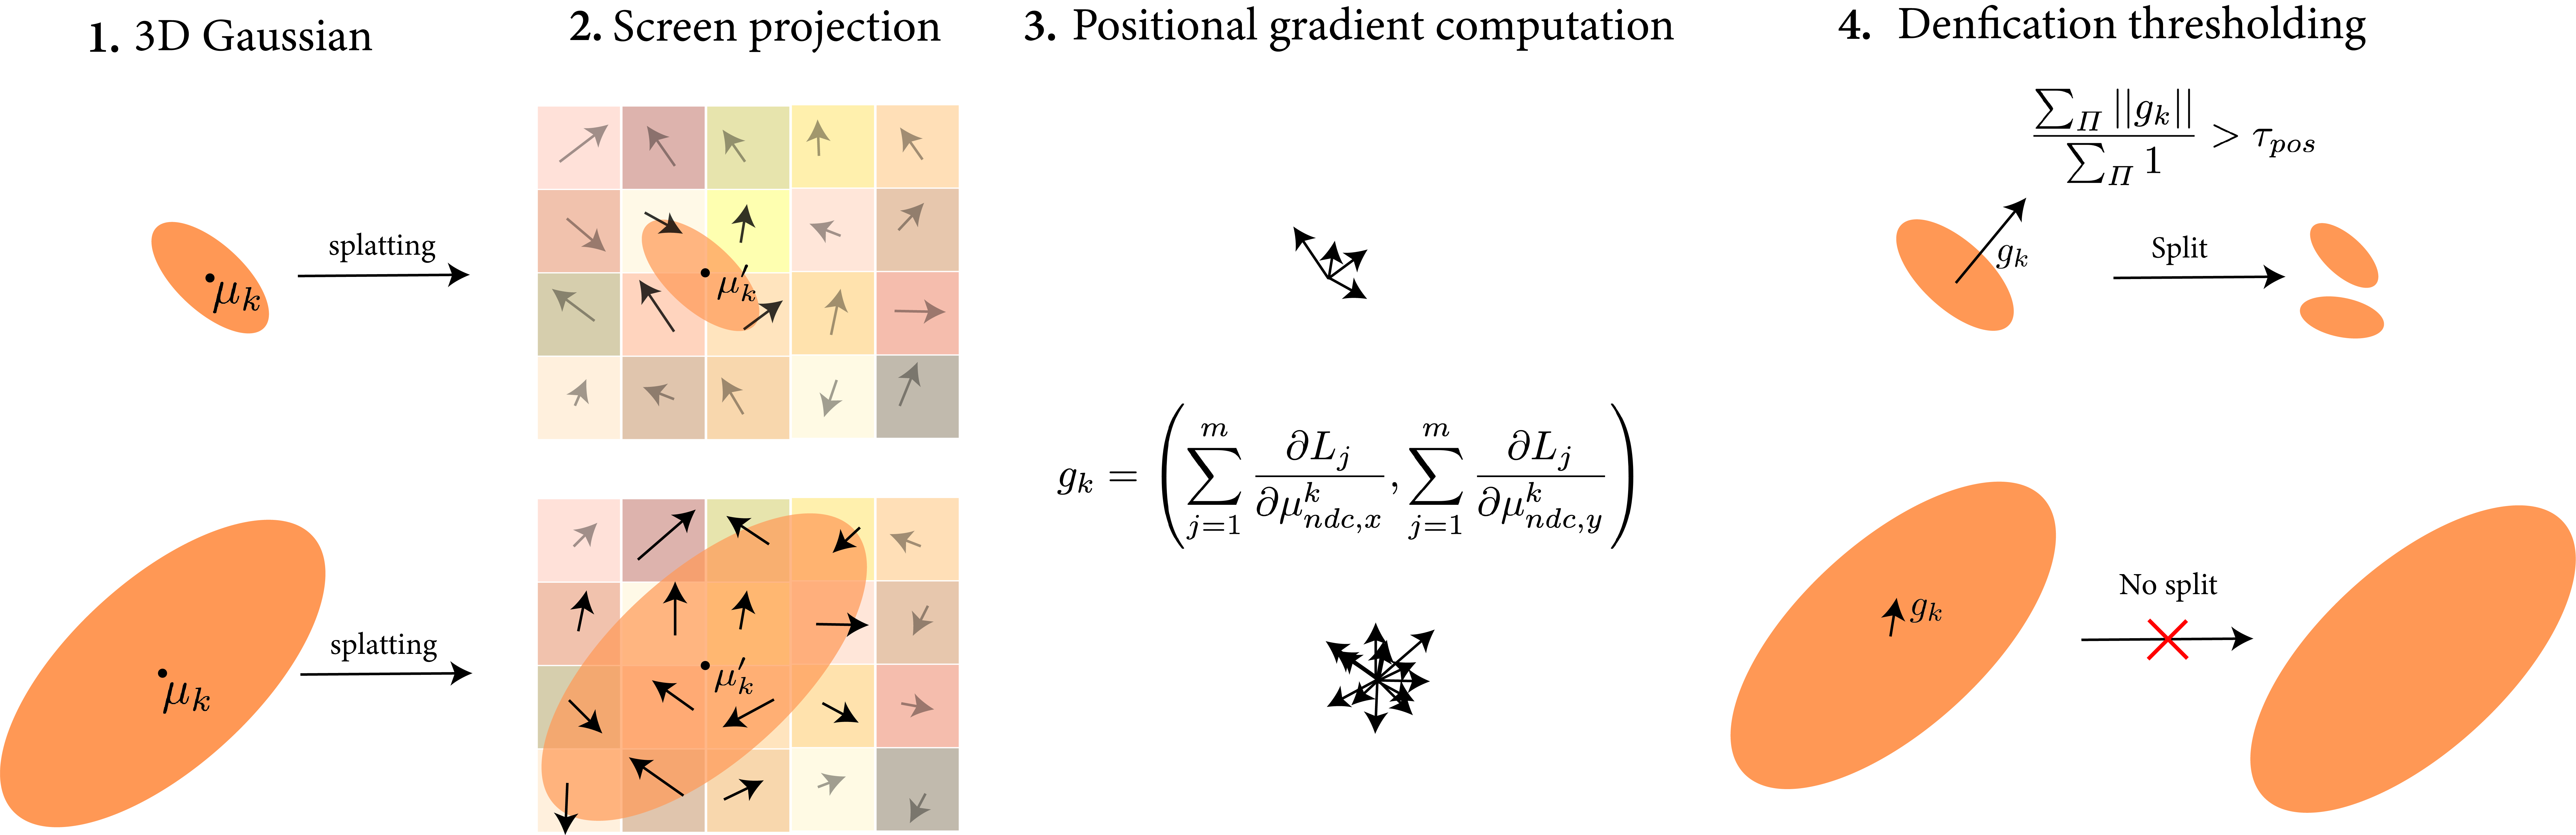
\includegraphics[width=\linewidth]{images/gaussiansplatting/adc_limitation.png}
  \caption{\textbf{ADC gradient collision.} It might occurred that large gaussians ends with low magnitude gradient, preventing the densification to happen.}
  \label{fig:adc-limitation}
\end{figure*}



To ease notation, we discard viewpoint $\pi$ and denote: 


\begin{equation}
\label{eq:grad-inter}
    g_{k,x} = \frac{\partial L}{\partial \mu^{k}_{ndc,x}} = \sum \limits_{j=1}^{m} \frac{\partial L_{j}}{\partial \mu^{k}_{ndc,x}} 
\end{equation}

% \begin{equation}
% \label{eq:grad-inter}
%     g_{k} = \left (\sum \limits_{j=1}^{m} \frac{\partial L_{j}}{\partial \mu^{k}_{ndc,x}} , \sum \limits_{j=1}^{m} \frac{\partial L_{j}}{\partial \mu^{k}_{ndc,y}} \right)
% \end{equation}

% \begin{equation}
% \frac{\sum_{\Pi} ||g_{k}||}{\sum_{\Pi} 1} > \tau_{pos}    
% \end{equation}

% \begin{equation}
% \frac{\sum_{\Pi} \textcolor{red}{m_{k}^{\pi}} ||g_{k}||}{\sum_{\Pi} \textcolor{red}{m_{k}^{\pi}}} > \tau_{pos}    
% \end{equation}
the x-axis gradient, with the per-pixel gradient expression: 

\begin{equation}
\label{eq:perpix-grad}
\frac{\partial L_{j}}{\partial \mu^{k}_{ndc,x}} = \sum \limits_{l=1}^{3} \frac{\partial L_{j}}{\partial c_{l}^{j}}\times \frac{\partial c_{l}^{j}}{\partial \alpha_{k}^{j}} \times \frac{\alpha_{k}^{j}}{\partial \mu^{k}_{ndc,x} }
\end{equation}

where $c_{l}^{j}$ refers to the color of the $l^{th}$ channel of the pixel $j$. The three different partial derivatives from equation (\ref{eq:perpix-grad}) might have different signs, affecting $\frac{\partial L_{j}}{\partial \mu^{k}_{ndc,x}}$  from equation (\ref{eq:grad-inter}). Complete proof can be found in the supplementary material. The more we sum over a large number of pixel, the more likely $\frac{\partial L}{\partial \mu^{k}_{ndc,x}}$ is prone to get closed to 0, preventing $\nabla_{\mu_{k}}L$ to be higher than $\tau_{pos}$ during the iteration cycle, as shown on Figure \ref{fig:adc-limitation}. 

PixGS tackles this gradient collision by re-weighting equation (\ref{eq:adc-original}) with the number of pixels $m_{k}$ covered by each primitives $\mathcal{G}_{k}$: 

\begin{equation}
\frac{\sum \limits_{\pi \in \Pi} m_{k}^{\pi} ||\frac{\partial L_{\pi}}{\partial \mu_{k}}||}{\sum \limits_{\pi \in \Pi}m_{k}^{\pi}} > \tau_{pos}
\label{eq:adc-original}
\end{equation}

PixelGS re-weighting strategy is illustrated on Figure \ref{fig:pixgs-adc}. 



\begin{figure*}[htbp!]
    \center
  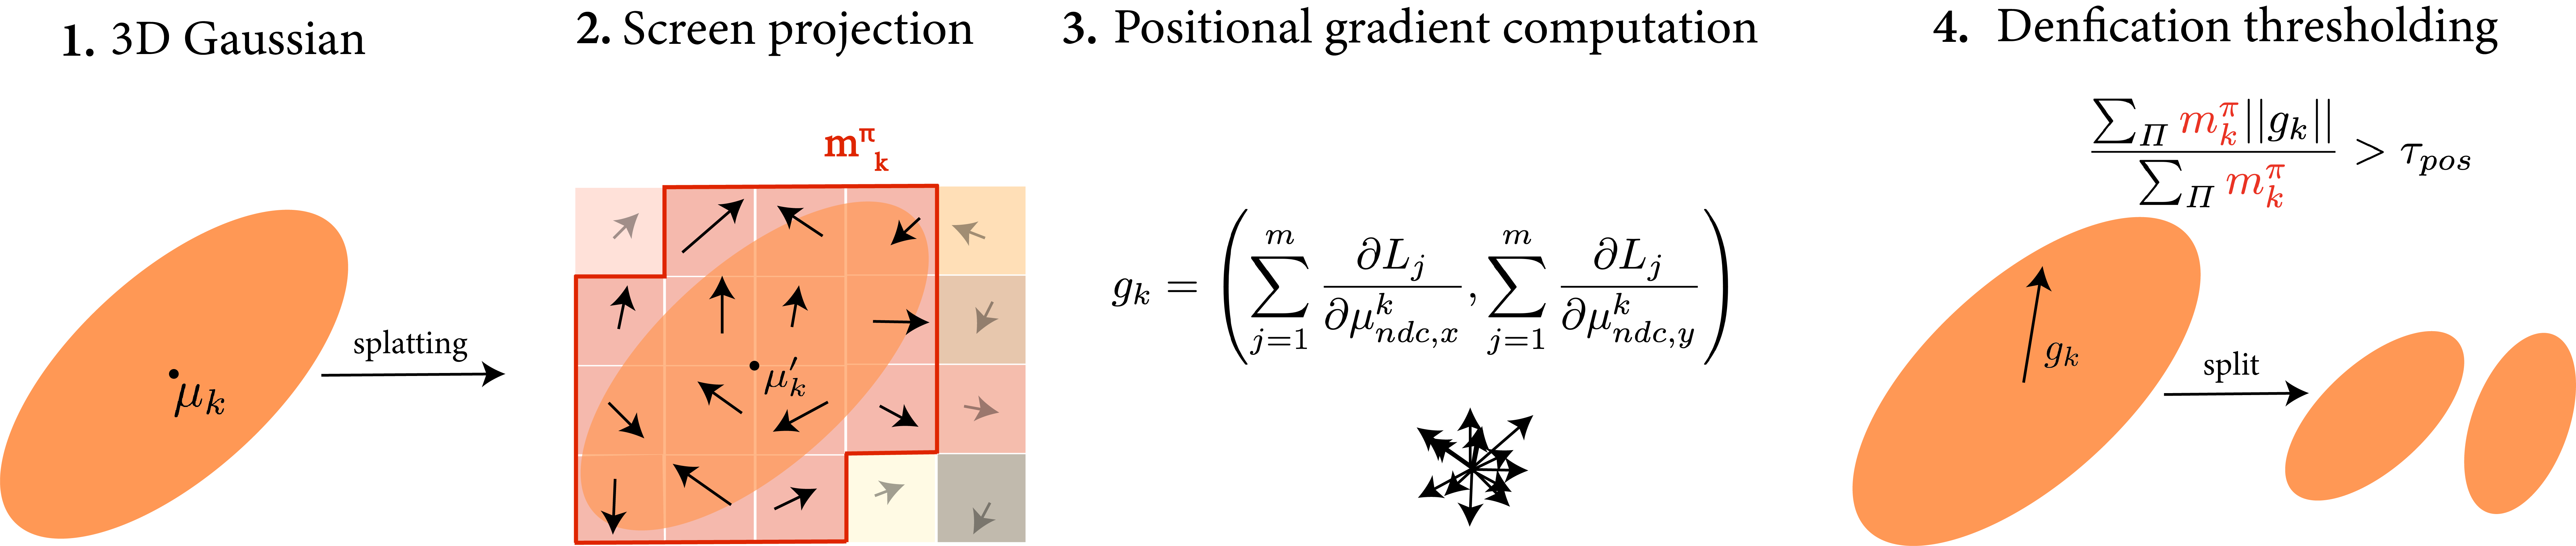
\includegraphics[width=\linewidth]{images/gaussiansplatting/pixgs_implem_improvement.png}
  \caption{\textbf{PixGS ADC correction.} By accounting on the number of pixel covered by a primitive, large gaussians have a higher gradient that is more likely to reach the density threshold $\tau_{pos}$}
  \label{fig:pixgs-adc}
\end{figure*}



\section{Experiments}
\label{sec:exp}

As our work has to be frame as a potential industrial system, all presented results come from the 36 views scene depicted on Figure \ref{fig:all_views}. 
\begin{figure*}[htpb!]
  \center
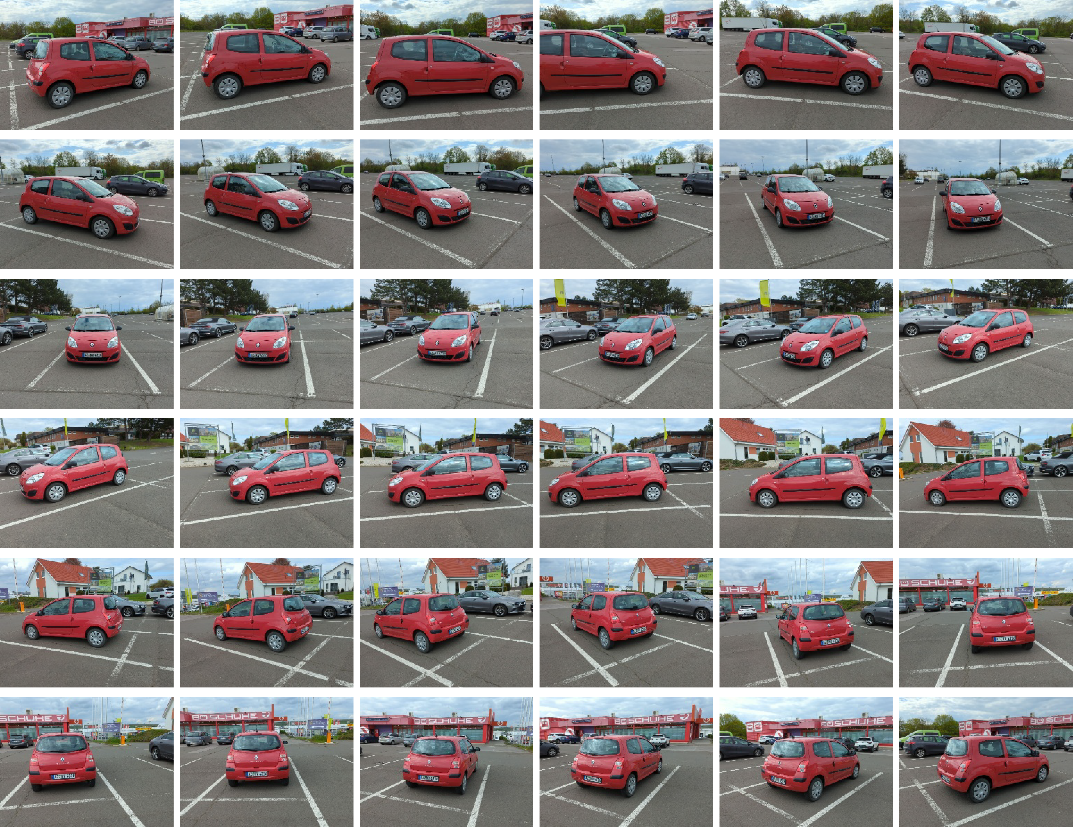
\includegraphics[width=.9\linewidth]{images/gaussiansplatting/original_scene.png}
\caption{\textbf{36 views $360^{\circ}$ spin scene.} Images has been acquired with a mobile device at $1500\times 2000$ resolution. As observed, car distance from the device objective is inconsistent across viewpoint.}
\label{fig:all_views}
\end{figure*}

We give visual insights and quantitative figures in this section to highlight how  each of the three modules we added to our GS system consistently improved the rendering quality. 

\subsection{Viewing Direction}

Additional MLP $\Phi$ that was added to our GS pipeline significantly improve transparent areas (such as windows) and highly specular regions, which cars are proned to.  We present a side by side comparison on Figure \ref{fig:gs-vh}. 


\begin{figure}[htb!]
  \centering
  \begin{subfigure}[b]{0.48\linewidth}
    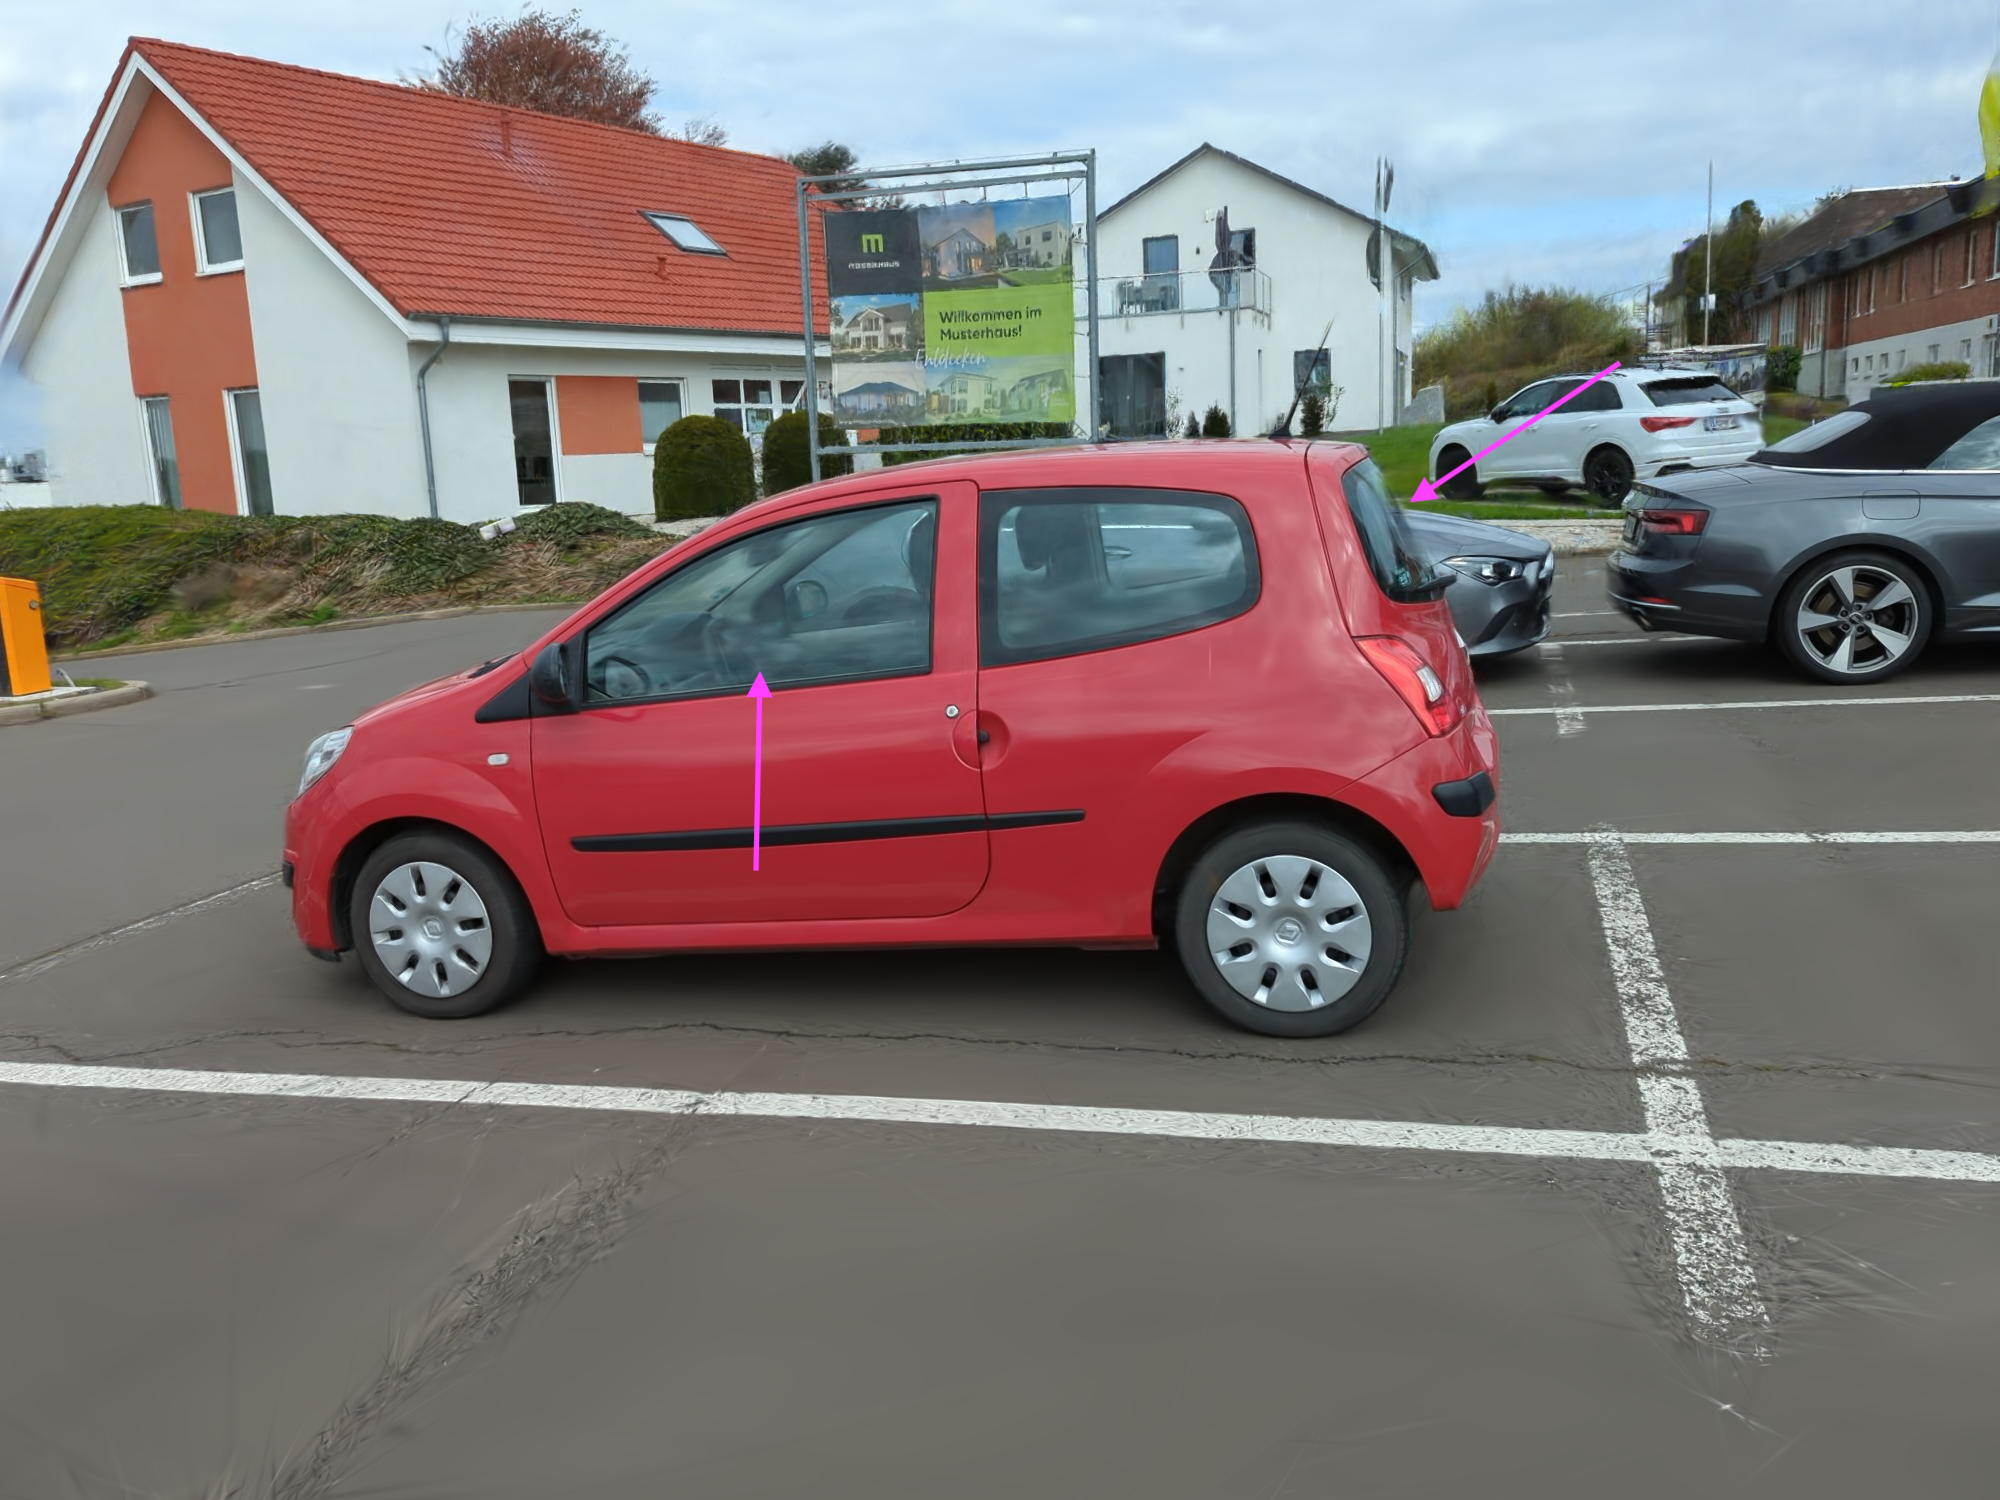
\includegraphics[width=\linewidth]{images/gaussiansplatting/00023-gs.png}
    \caption{\textbf{Vanilla GS rendering view}}
    \label{fig:view3}
  \end{subfigure}
  \quad % Space between the figures
  \begin{subfigure}[b]{0.48\linewidth}
    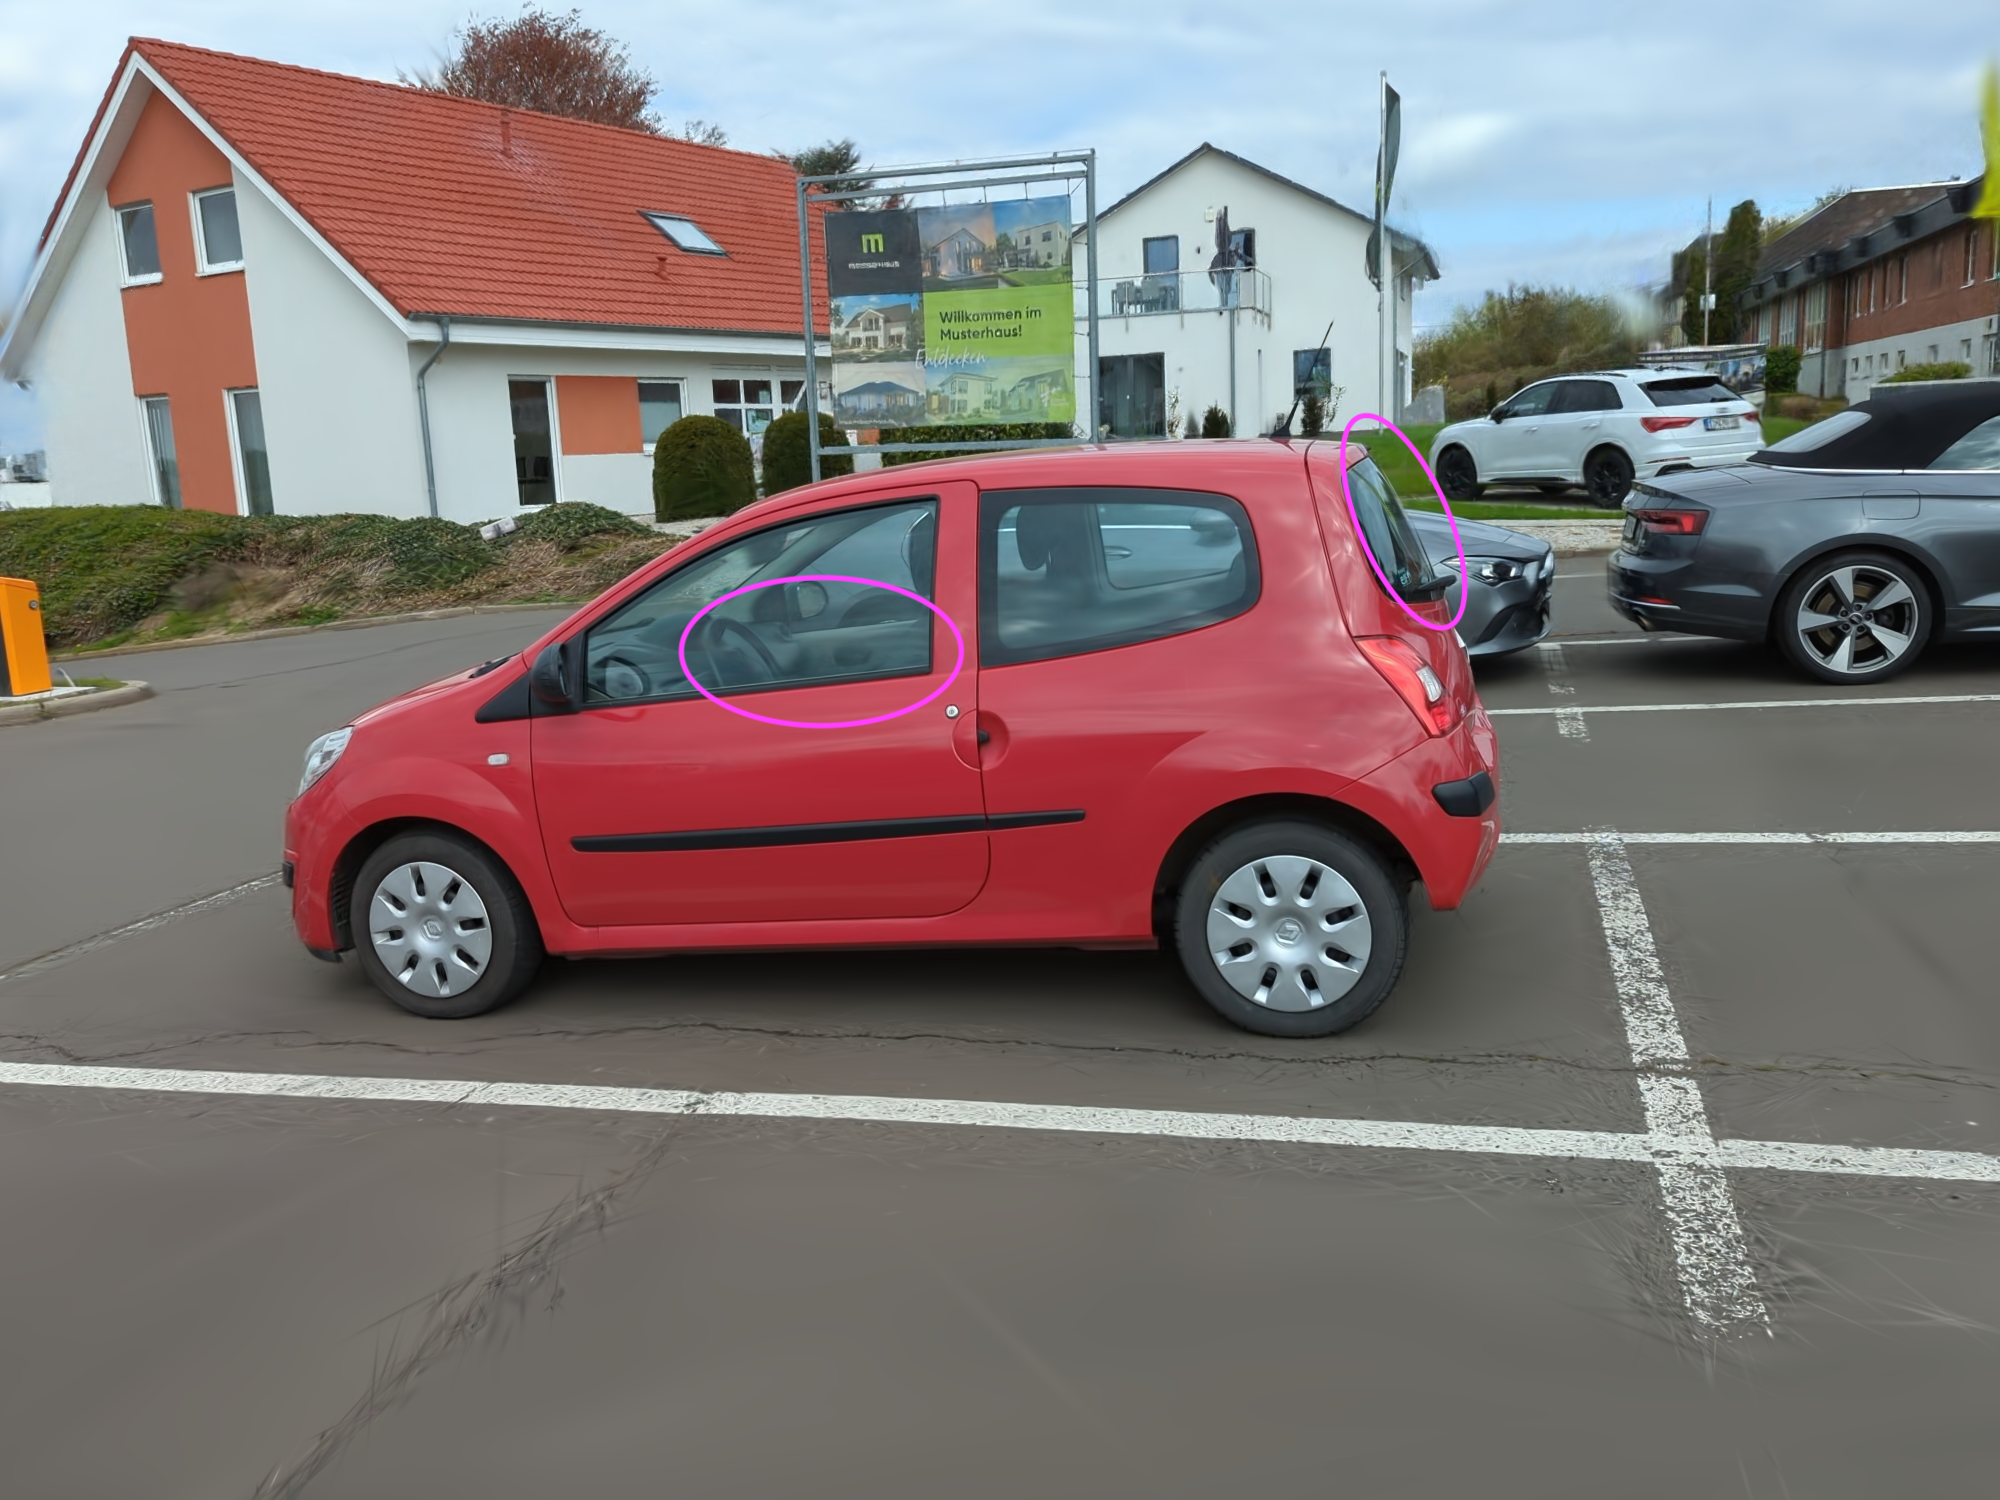
\includegraphics[width=\linewidth]{images/gaussiansplatting/00023-gs-vd.png}
    \caption{\textbf{With Viewing Direction MLP}}
    \label{fig:gs-view3-gs}
  \end{subfigure}
  \caption{\textbf{Viewing Direction influence.} Whereas vanilla Gaussian Splatting code struggles with reflective and transparent regions, adding such an MLP before the rasterization significantly improve rendering results. }
  \label{fig:gs-vh}
\end{figure}



\subsection{Visual hull} 

We present on Figure \ref{fig:gs-vishull-comp} three renderings of the same view but from three different trained scene. First scene was trained with the original point cloud procuded by the COLMAP-SfM algorithm, second with the VisHull point cloud while the latest get consideration for merging both COLMAP-SfM and VisHull point cloud together.   



\begin{figure*}[htb!]
  \center
\includegraphics[width=\linewidth]{images/gaussiansplatting/vishull_ablation.png}
\caption{\textbf{Point cloud initilization influence.} COLMAP-based point \textit{(left)},visual hull based \textit{(center)} and merged point clouds \textit{(right)}  rendering result.}
\label{fig:gs-vishull-comp}
\end{figure*}


COLMAP-SfM based rendering yields a satisfying result, even though some inner details are missed. The visual hull based initialization method produce sharper results in the car, but floaters are rendered on the roof the car. Merging the two point cloud \textit{(right)} allows to get the best of both configuration. 

These visual improvement on the rendered views are quantitatively confirmed through the whole training set with the three metrics we used to assess the rendering quality. Results are gathered in Table \ref{table:gs-vh-influence}. Figures tend to highlight a phenomena that was highly expected: as soon as no points are affected in the background regions at the initialisation stage with the \textit{VisualHull} configuration, the latter is weaker than the \textit{COLMAP-SfM} based setting at rendering clear background. Such a limitation is quantatively confirmed in the figures: results from \textit{VisualHull} configuration are better when metrics are only computed on the car. 
\begin{table}[htp!]
  \caption{\textbf{VisualHull influence.} Quantitative results how influenciable the original point cloud can be on the GS rendering performance.}
  \label{table:gs-vh-influence}
  \begin{adjustbox}{width=\linewidth}
  \begin{tabular}[h]{c||ccccccc}
  \hline
   PC initialization & \multicolumn{3}{c}{Full Image} & \multicolumn{3}{c}{Car only} \\
   &  SSIM ($\uparrow$) & PSNR ($\uparrow$) & LPIPS ($\downarrow$) & SSIM ($\uparrow$) & PSNR ($\uparrow$) & LPIPS ($\downarrow$)\\
  \hline
  COLMAP-SfM \textit{only} & 0.808 & 29.163 & 0.318 & 0.983 & 40.917 & 0.031\\
  VisualHull \textit{only} & 0.764 & 27.254 & 0.373 & 0.980 &   39.271 & 0.035 \\
  COLMAP-SfM + VisualHull & \textbf{0.810} & \textbf{29.288} & \textbf{0.314}  & \textbf{0.984} & \textbf{41.249}   & \textbf{0.030} \\
  \hline 
  \end{tabular}
  \end{adjustbox}
  \end{table}


\subsection{PixGS ADC} 

We finally highlight the  positive impact a clever adaptive density control have. Qualitative results are shown in Figure \ref{fig:gs-pigs}. 


\begin{figure}[htb!]
  \centering
  \begin{subfigure}[b]{0.45\linewidth}
    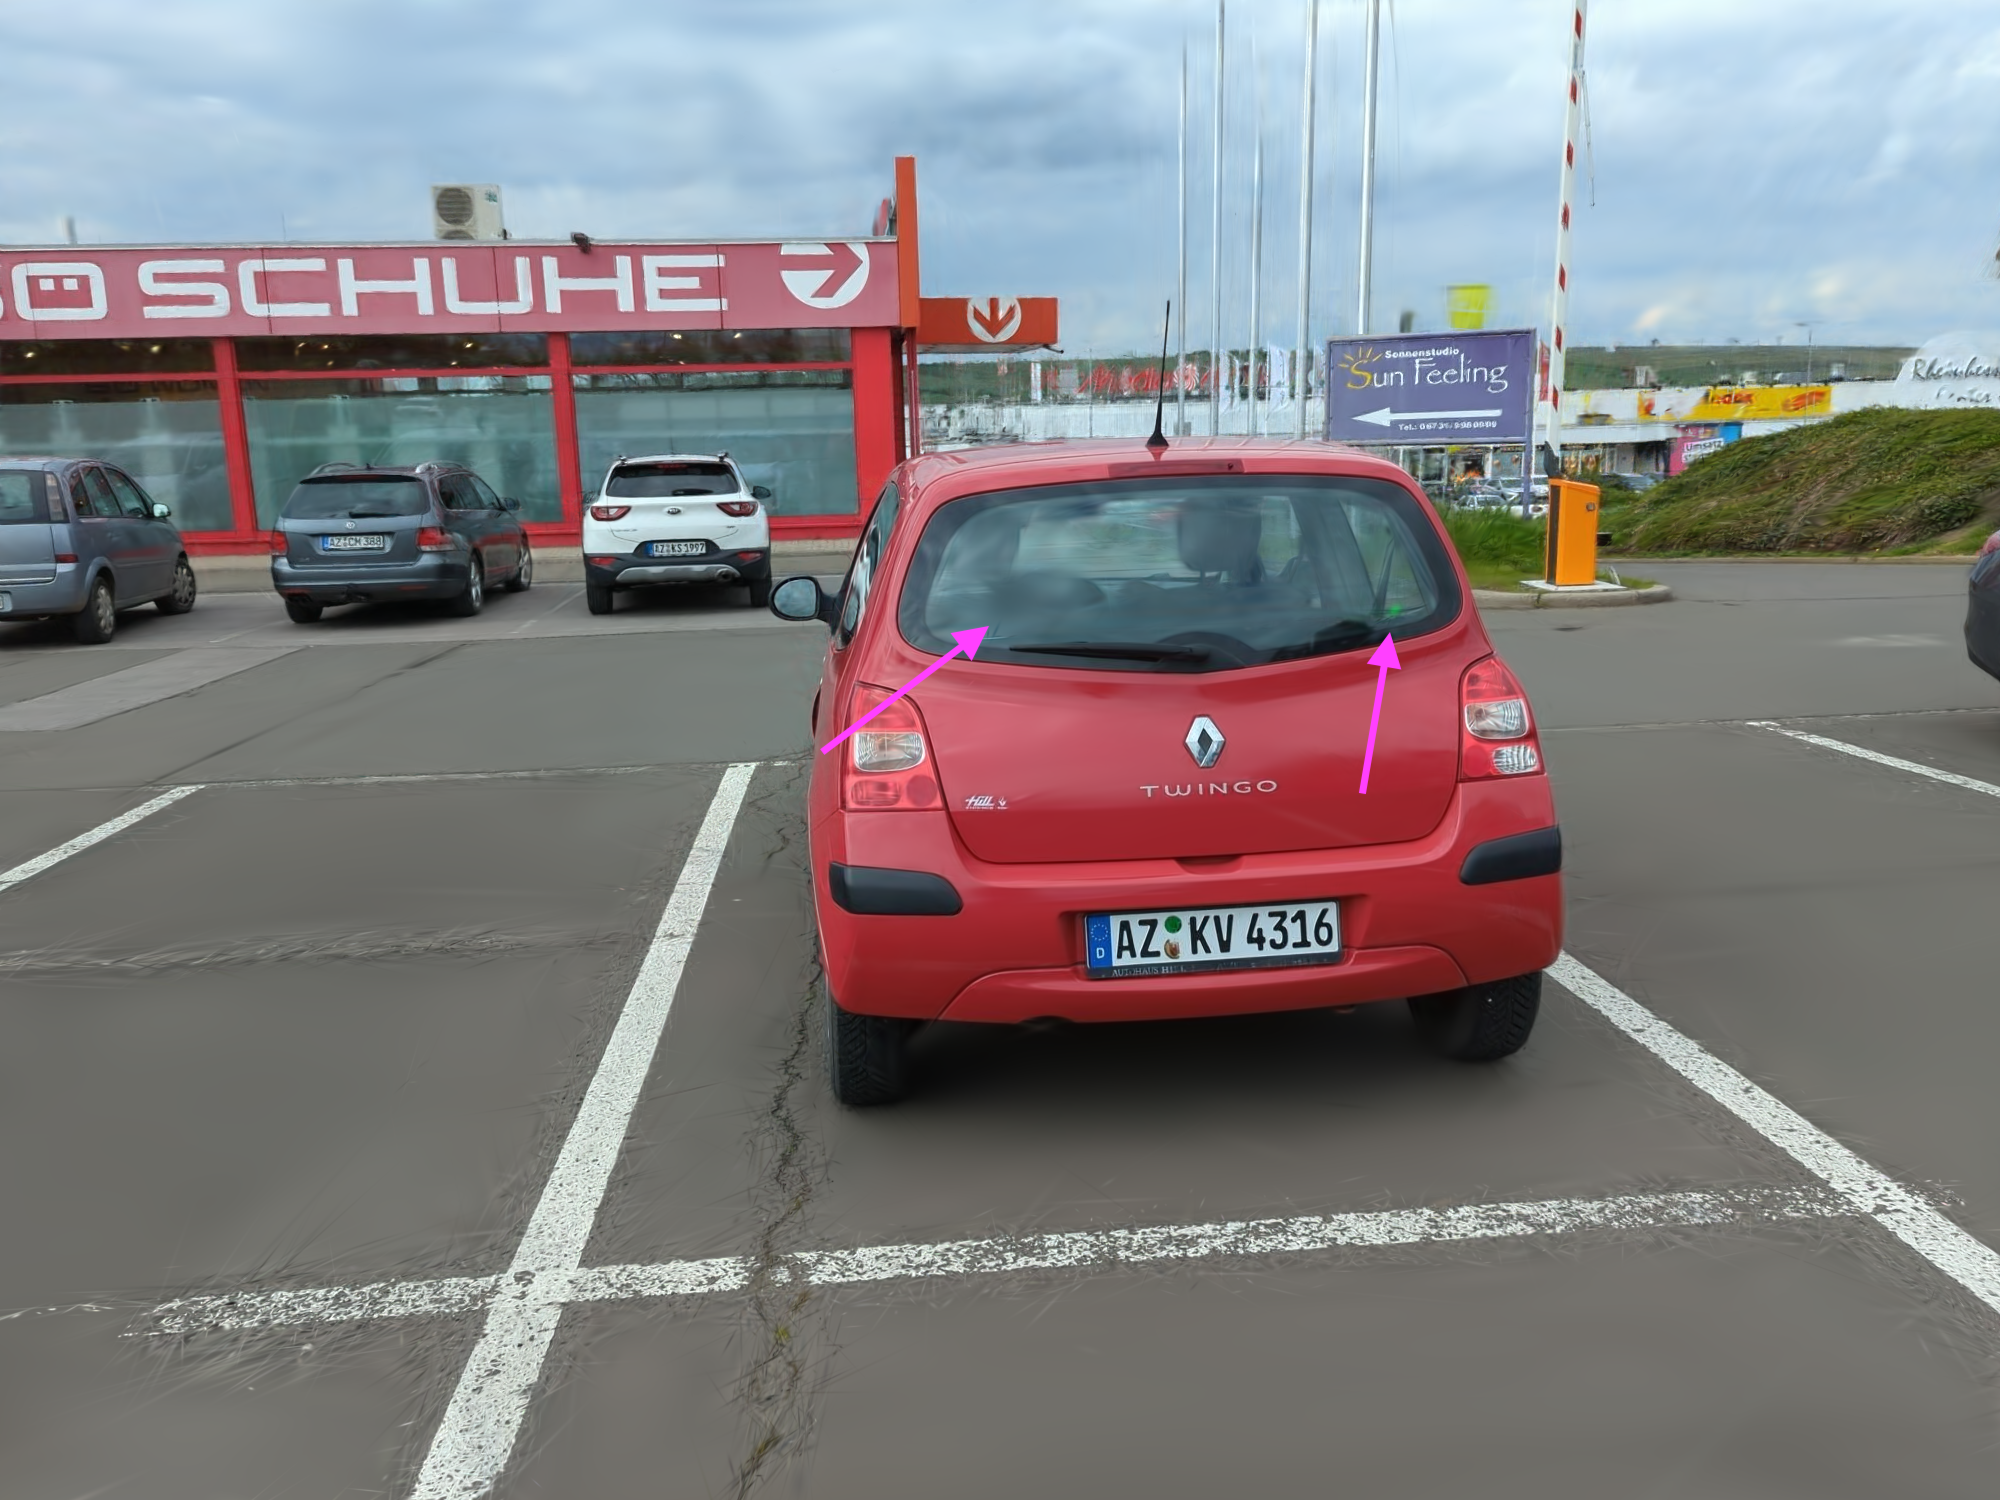
\includegraphics[width=\linewidth]{images/gaussiansplatting/00029-gs.png}
    \caption{\textbf{Vanilla GS rendering view}}
    \label{fig:view3}
  \end{subfigure}
  \quad % Space between the figures
  \begin{subfigure}[b]{0.45\linewidth}
    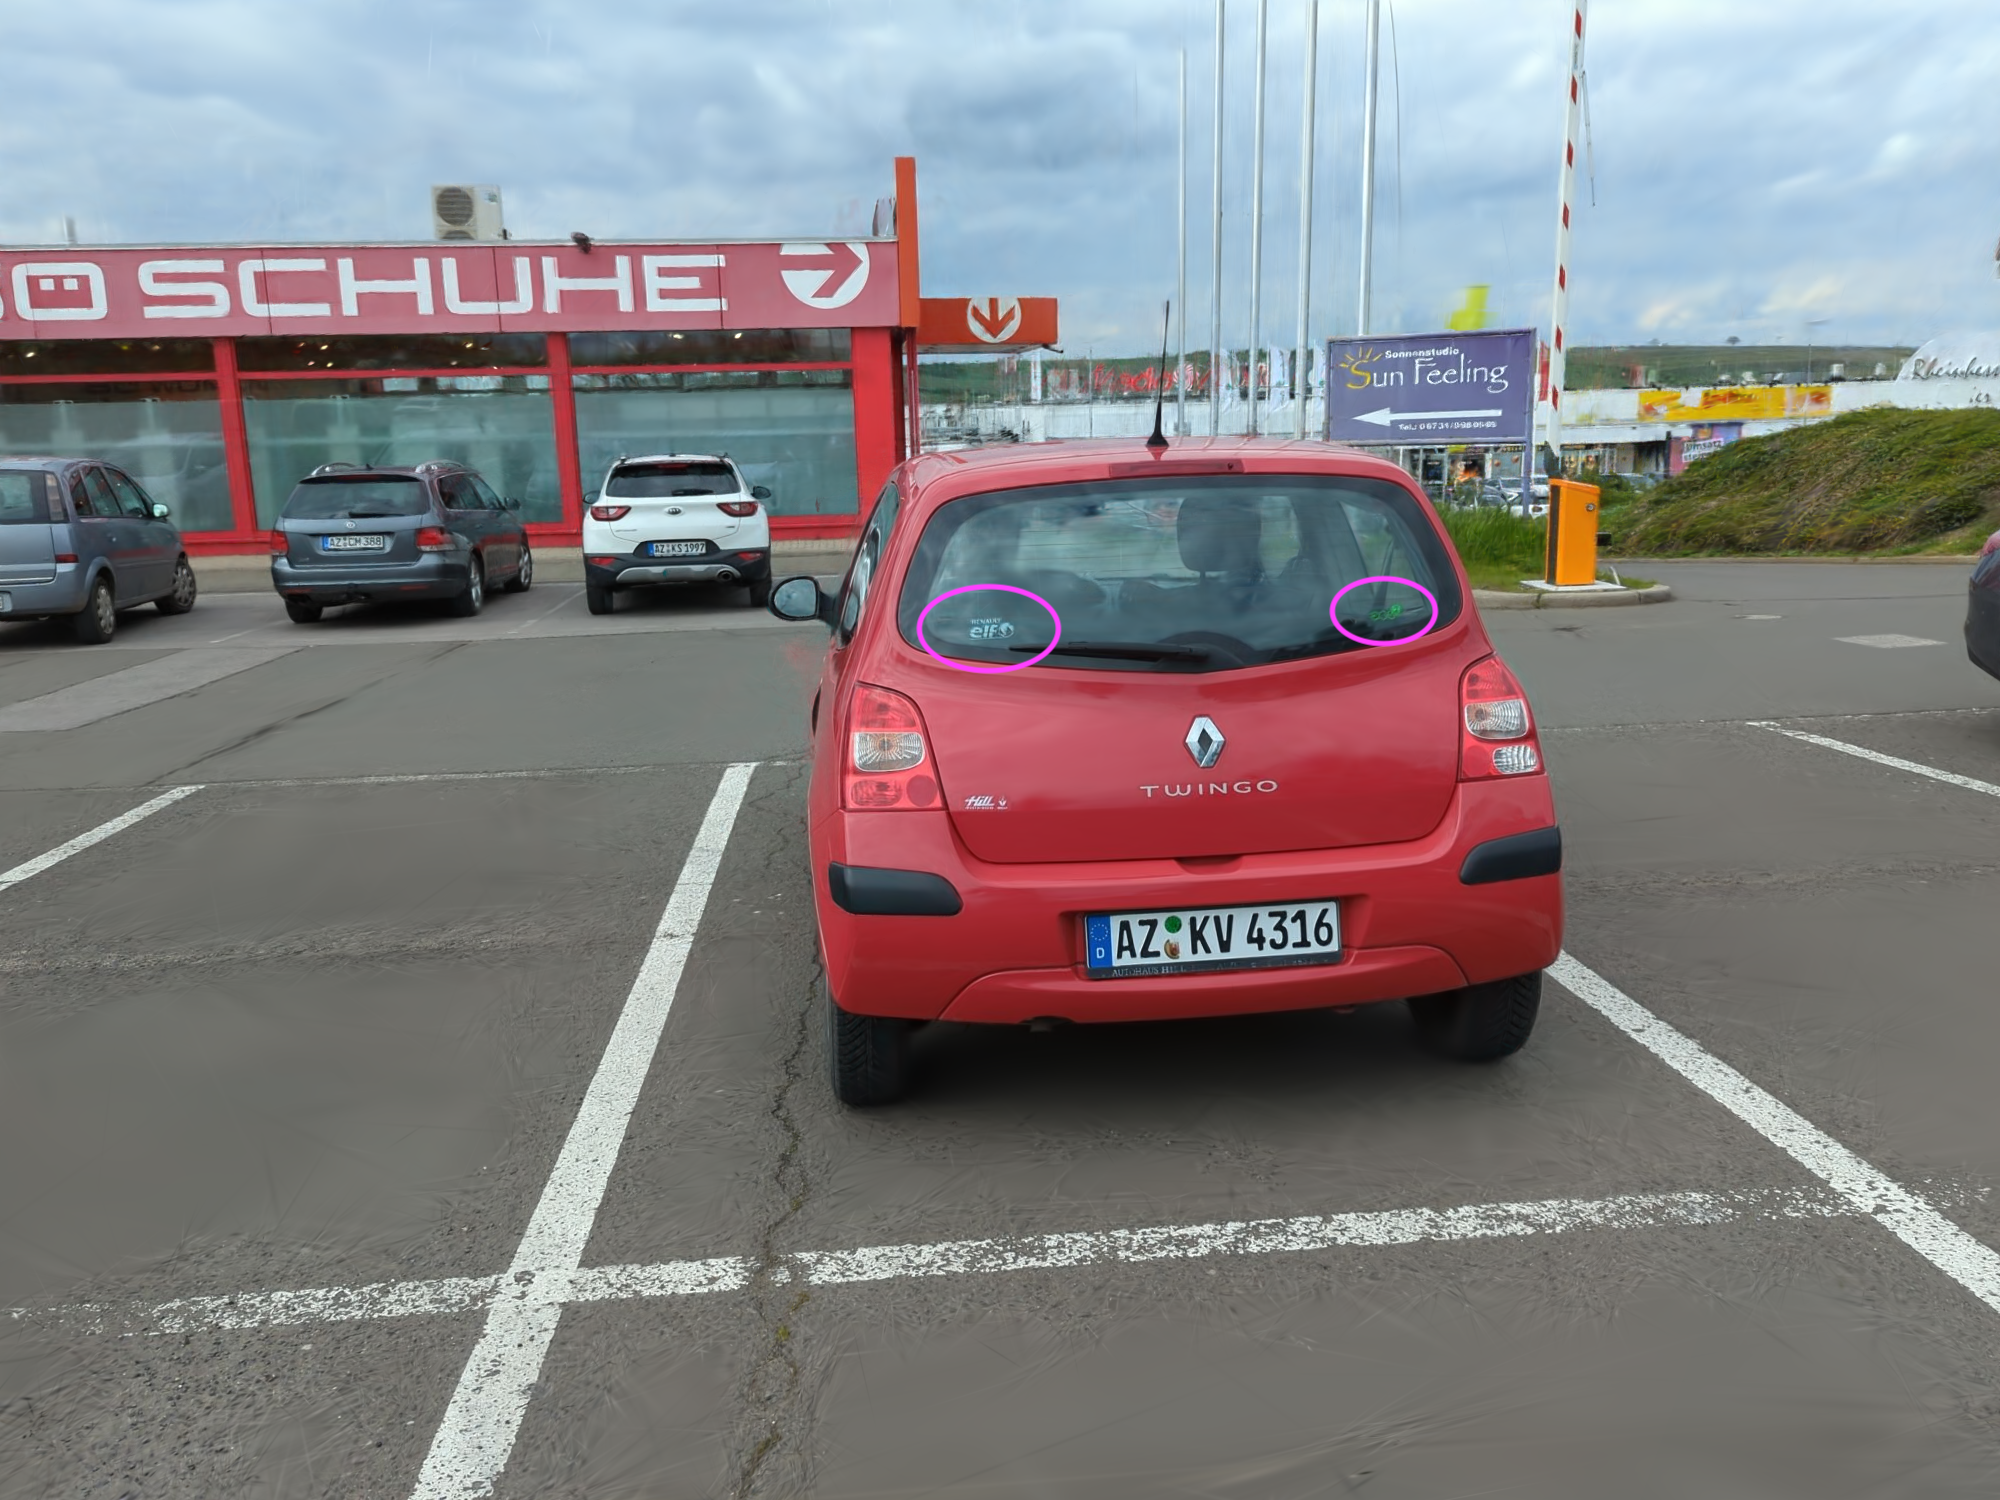
\includegraphics[width=\linewidth]{images/gaussiansplatting/00029-pixgs.png}
    \caption{\textbf{PixGS rendering view}}
    \label{fig:gs-view3-gs}
  \end{subfigure}
  \caption{\textbf{PixGS Adaptative Density Control influence.} Both logo on the rear windows are missing on the vanilla GS version: nor the \textit{Renault elf} and \textit{ECO} sign are visible. PixGS, through its clever densification strategy, managed to render such tiny details.}
  \label{fig:gs-pigs}
\end{figure}

Only core difference PixGS has over the vanilla GS implementation is the \ac{ADC} component. As soon as such a component is replaced in our system, rendered views immediately gain in sharpness and details: over and under- reconstructed areas are better handle by the \ac{ADC} module. Nor the viewing direction MLP or the visual hull initialisation were used here. 

\subsection{Complete pipeline}

We finally conduct a complete ablation study over our different modules to emphasize on the consistency each of our modifications bring to the entire GS pipeline system. 

Table \ref{table:gs-abaltion} summarises the impact each of our module has. Whereas both the viewing direction MLP and the PixGS densification strategy steadily enhance all our metrics, the visual hull has only a limited impact outside the car region. Such an observation is in line with what was already observed in figures from Table \ref{table:gs-abaltion}. 

\begin{table}[htp!]
  \caption{\textbf{Ablation study.} Influence of our different algorithm components on our $360^{\circ}$ GS system.}
  \label{table:gs-abaltion}
  \begin{adjustbox}{width=\linewidth}
  \begin{tabular}[h]{c||ccccccc}
  \hline
   Pipeline & \multicolumn{3}{c}{Full Image} & \multicolumn{3}{c}{Car only} \\
   &  SSIM ($\uparrow$) & PSNR ($\uparrow$) & LPIPS ($\downarrow$) & SSIM ($\uparrow$) & PSNR ($\uparrow$) & LPIPS ($\downarrow$)\\
  \hline
  GS \cite{kerbl20233d}  & 0.798  & 28.413 & 0.325 & 0.980 & 38.668 & 0.036 \\
  + Viewing Direction & 0.808 & 29.163 & 0.318 & 0.983 & 40.917  & 0.031 \\
  + VisualHull & 0.810 & 29.288 & 0.314 & 0.984 &41.249  & 0.030 \\
  + PixGS \ac{ADC} & \textbf{0.861} & \textbf{31.077} & \textbf{0.248} & \textbf{0.990} & \textbf{43.983} & \textbf{0.020} \\
  \hline 
  \end{tabular}
  \end{adjustbox}
  \end{table}

These figures are finally visually confirmed through the exhaustive rendered views depicted on Figure \ref{fig:gs-vh-result}. As one could observed, the original GS code fails on this rendered view to retrive tiny and complex details as the tank fuel or the car interior. Adding the viewing direction MLP $\Phi$ before the rasterizing stage helps the training of our system a lot. Corresponding rendered view has now a better car interior, whereas the fuel tank is still partially rendered. On top of this first modification, merging both the visual hull point cloud with the one produced by COLMAP helped the GS training: car exterior and interior details has been preserved and even improved. The tank fuel is now almost entirely rendered. Finally, the densification strategy proposed by PixGS is striking regarding car details. Fuel tank is perfectly rendered but car interior is now extremely well rendered and one could struggle to distinguish the real ground truth image from the rendered one by only focusing on the car itself.   

\begin{figure*}[htb!]
  \center
\includegraphics[width=\linewidth]{images/gaussiansplatting/image_final.png}
\caption{\textbf{Cumulative influence of our different module} Each module that was implemented in our system consistently bring its own contribution without deteriorating what was improved by former algorithm brick. Car interior and fuel tank details are progressively improved until our final system model.}
\label{fig:gs-vh-result}
\end{figure*}

\section{Limitation and further works}

Wheareas our 3D reconstruction pipeline is able to faithfully render and synthesize novel view at training and \textit{in-distribution} locations, moving to far war away from the original camera path might lead to severe artefact at render time. One of the most known undesired effect for 3D \ac{GS} scene is so-called floater artifact. We illustrate on Figures \ref{fig:floater-limitation} and \ref{fig:floater-removed} this effect\footnote{We illustrate this limitation on another scene since the one we used in this chapter is not that much prone to such needle artifact effect.} and how it can easely handled by narrowing the viewing camera frustrum at inference time. These needle artifacts are rendered when $z_{min}=0.2$ since the associated gaussians primitives has the minimal required depth to be taken into account during the rasterization. Increasing the minimal depth to $z_{min}=1.2$ each primitive has to get for being rasterized allow to not render them anymore since they do not fall into the new camera frustrum that has been narrowed. 

\begin{figure*}[htb!]
  \center
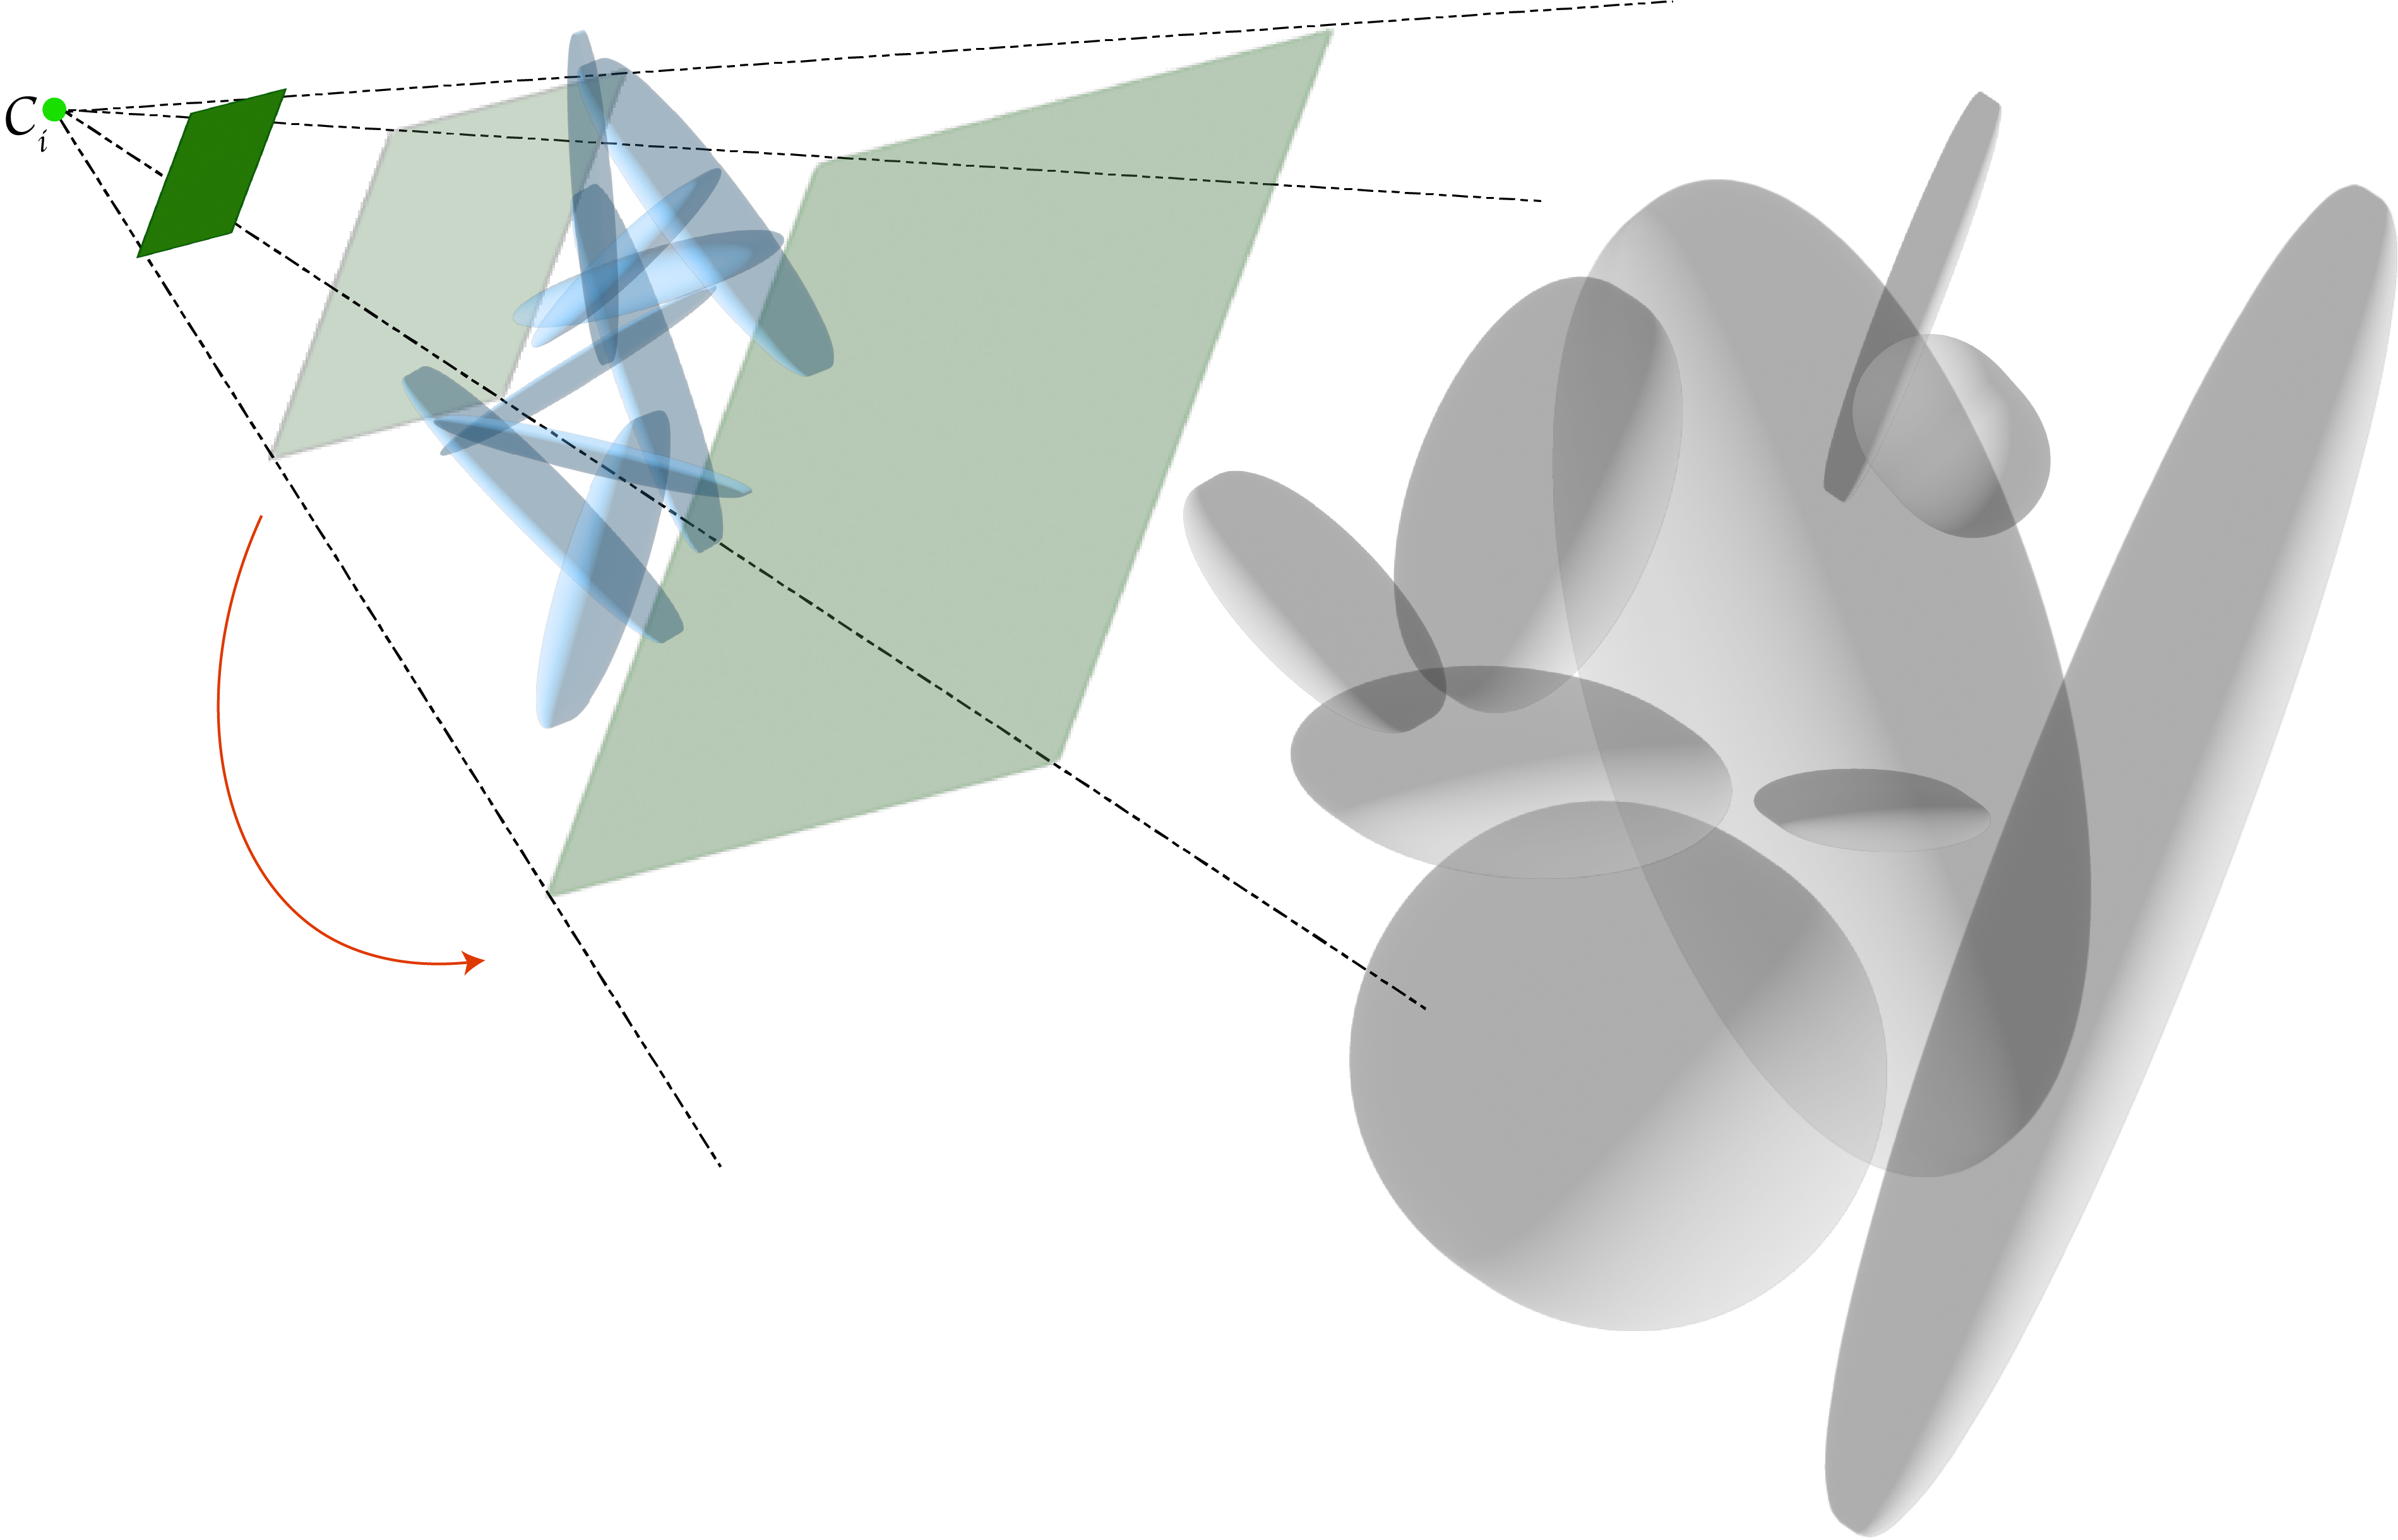
\includegraphics[width=.7\linewidth]{images/gaussiansplatting/gaussian-floaters.png}
\caption{\textbf{Toy illustration for camera frustrum narrowing} Increasing the minimal depth at which gaussian primitives are rasterized or not allows to avoid undesired gaussians being rendered at non-training locations.}
\label{fig:floater-limitation}
\end{figure*}

\begin{figure}[htb!]
  \centering
  \begin{subfigure}[b]{0.45\linewidth}
    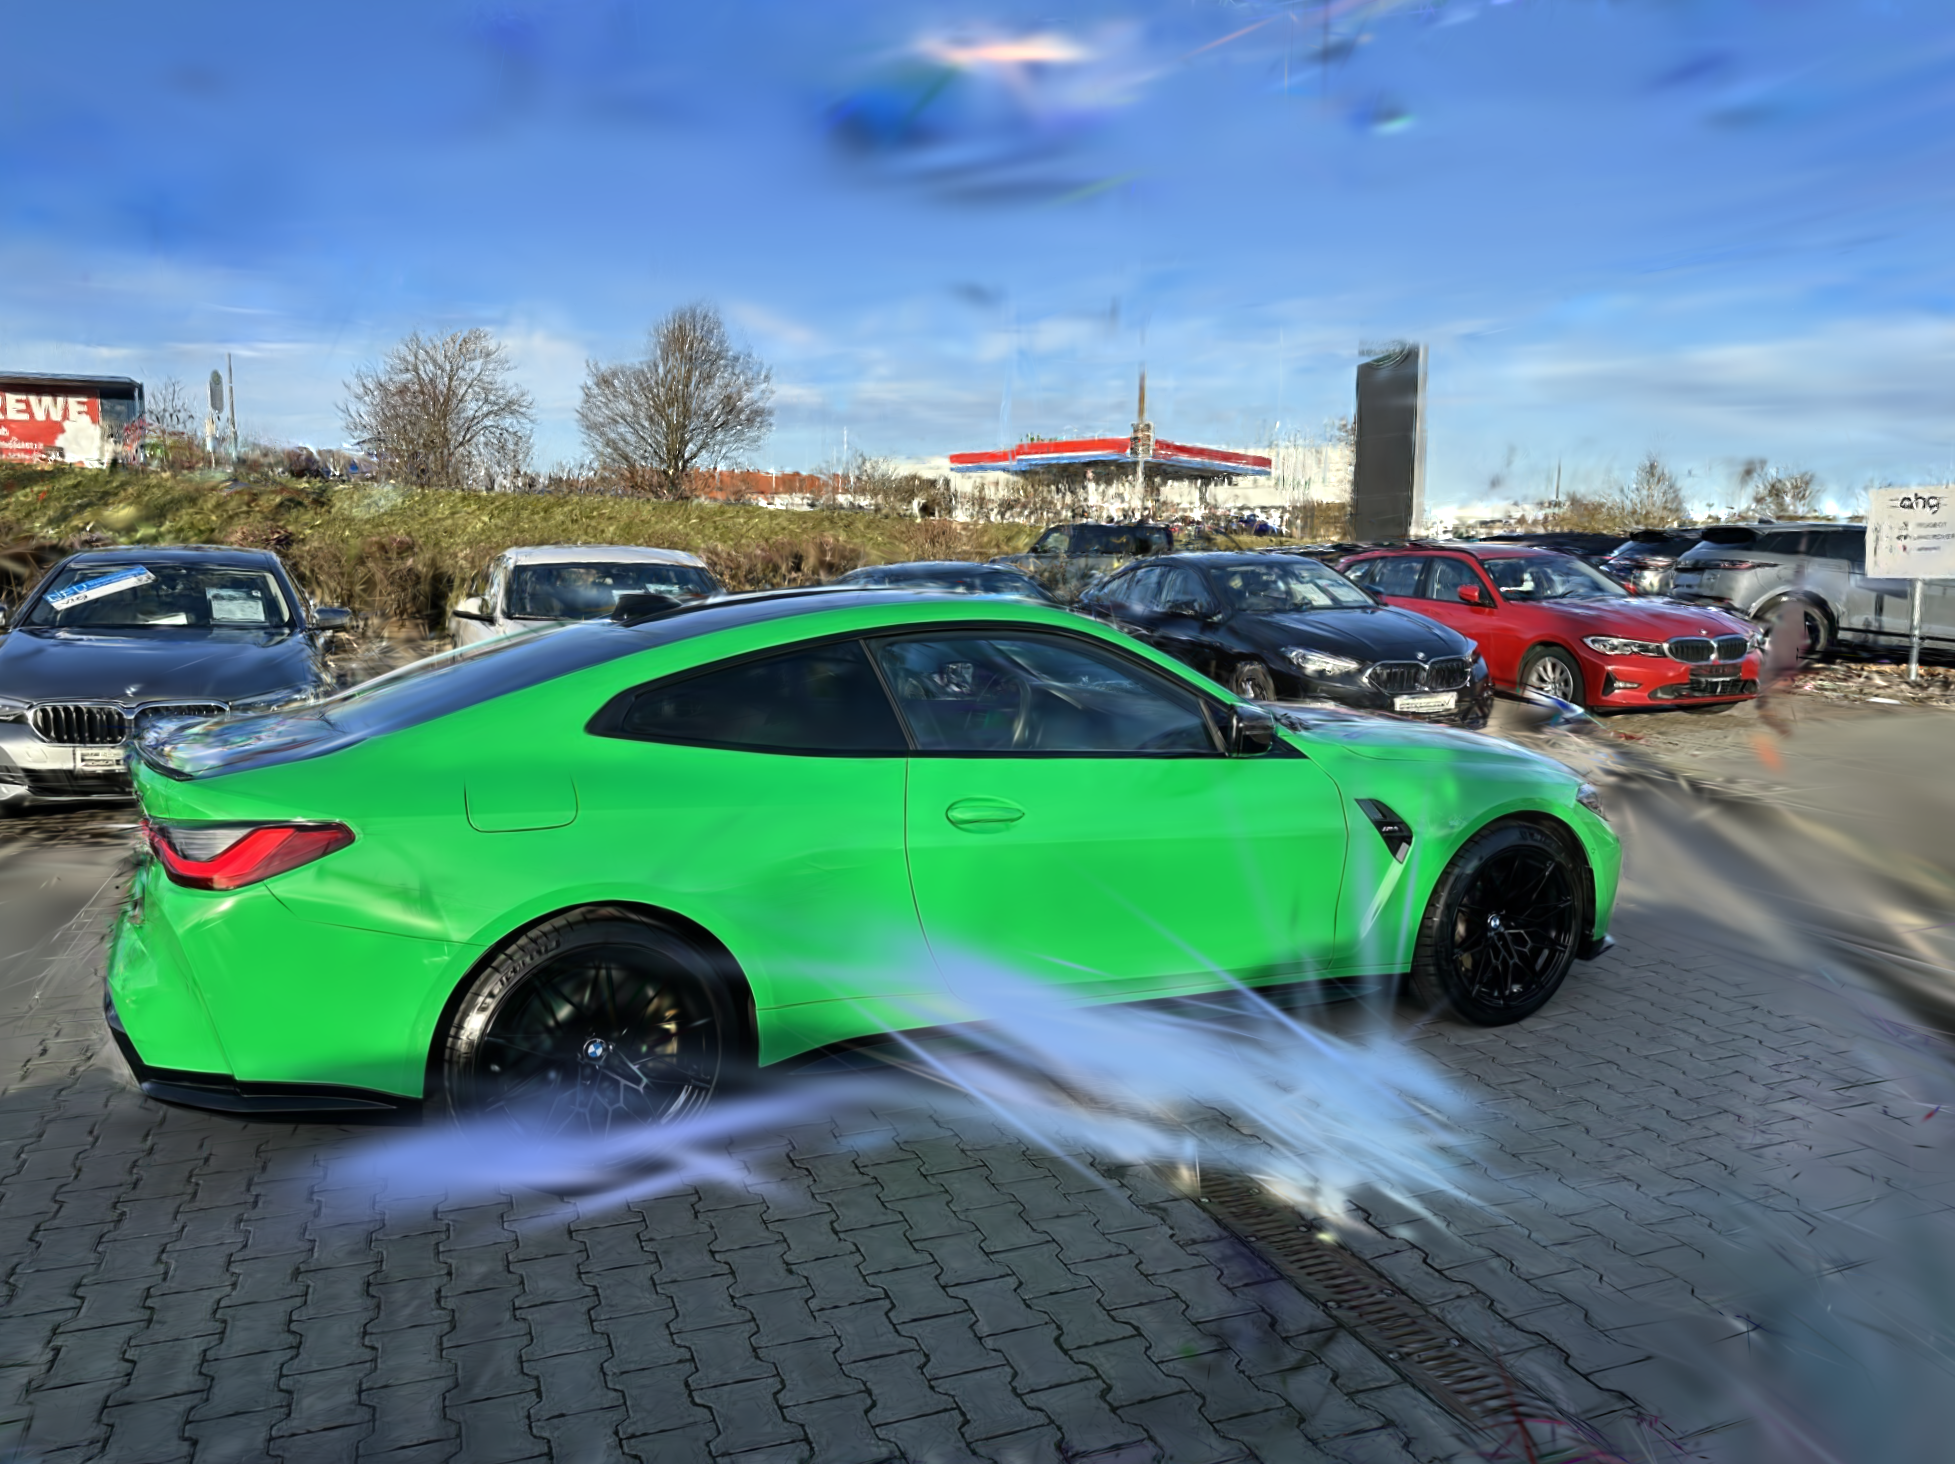
\includegraphics[width=\linewidth]{images/gaussiansplatting/needle-artifact.png}
    \caption{\textbf{Rendering with $z_{min}$=0.2} }
  \end{subfigure}
  \quad % Space between the figures
  \begin{subfigure}[b]{0.45\linewidth}
    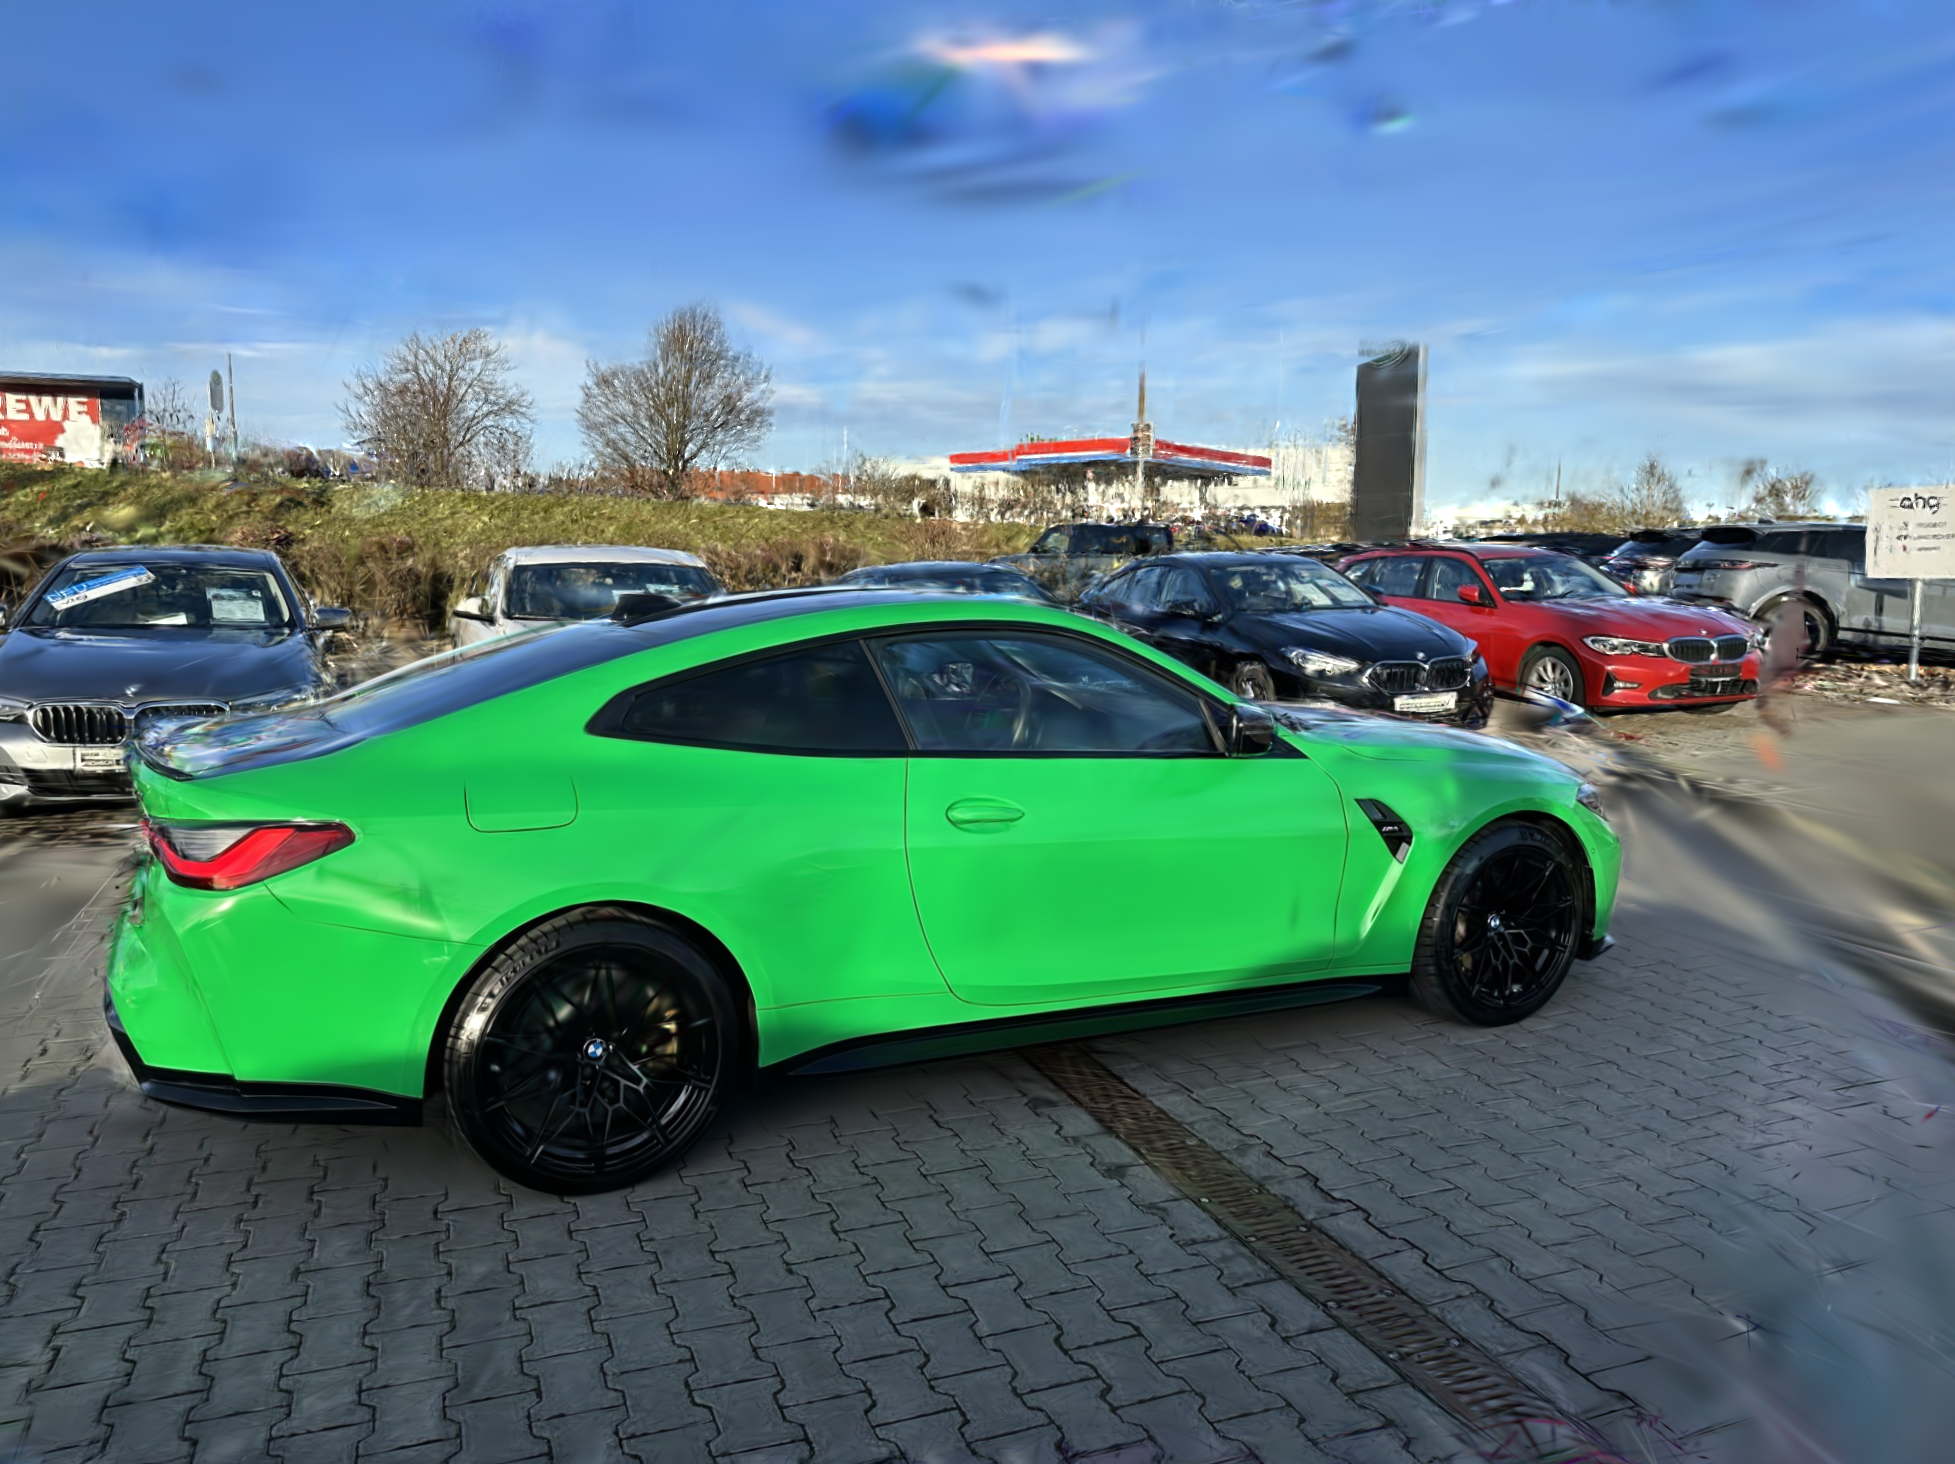
\includegraphics[width=\linewidth]{images/gaussiansplatting/needle-free-artifact.png}
    \caption{\textbf{Rendering $z_{min}$=1.2} }
  \end{subfigure}
  \caption{\textbf{Camera frustrum impact onto needle artifact rendering.} Slightly changing the minimal depth value at which gaussian primitives are rendered or not on the image plane has a huge impact on the final image. Increasing such minimal depth value allows to get ride of those needle primitives when one need to render at a location that is behind the original training location.}
  \label{fig:floater-removed}
\end{figure}

Beyond the rendering of these unwanted gaussian primitives, rendering at non-training locations remains a challenging tak that would need to be handle during further research. Indeed, only having a sparse set of 36 views to reconstruct a whole scene remains a challenging task: public datasets on which \ac{GS} is trained on for academic purposes often have few hundreds of input images. The figure \ref{fig:nontraining-rendering} illustrates the common case we faced when we need to stabilize the $360^{\circ}$ spin of this scene. The view has to be rendered at a location that is slighly above the original training view. The 3D \ac{GS} scene is extremely well rendered at this training location, at least on the car itself (while the ground and the sky suffer from a lack of gaussian primitives in those over-reconstructed regions). Moving toward the car, at a non-training location, lead to a rendering that is far from being acceptable for an industrial application. Several artifacts and misplaced / misoriented gaussians appeared on the back of the car, leading to an blurry and fuzzy result. 

\begin{figure}[htb!]
  \centering
  \begin{subfigure}[b]{0.45\linewidth}
    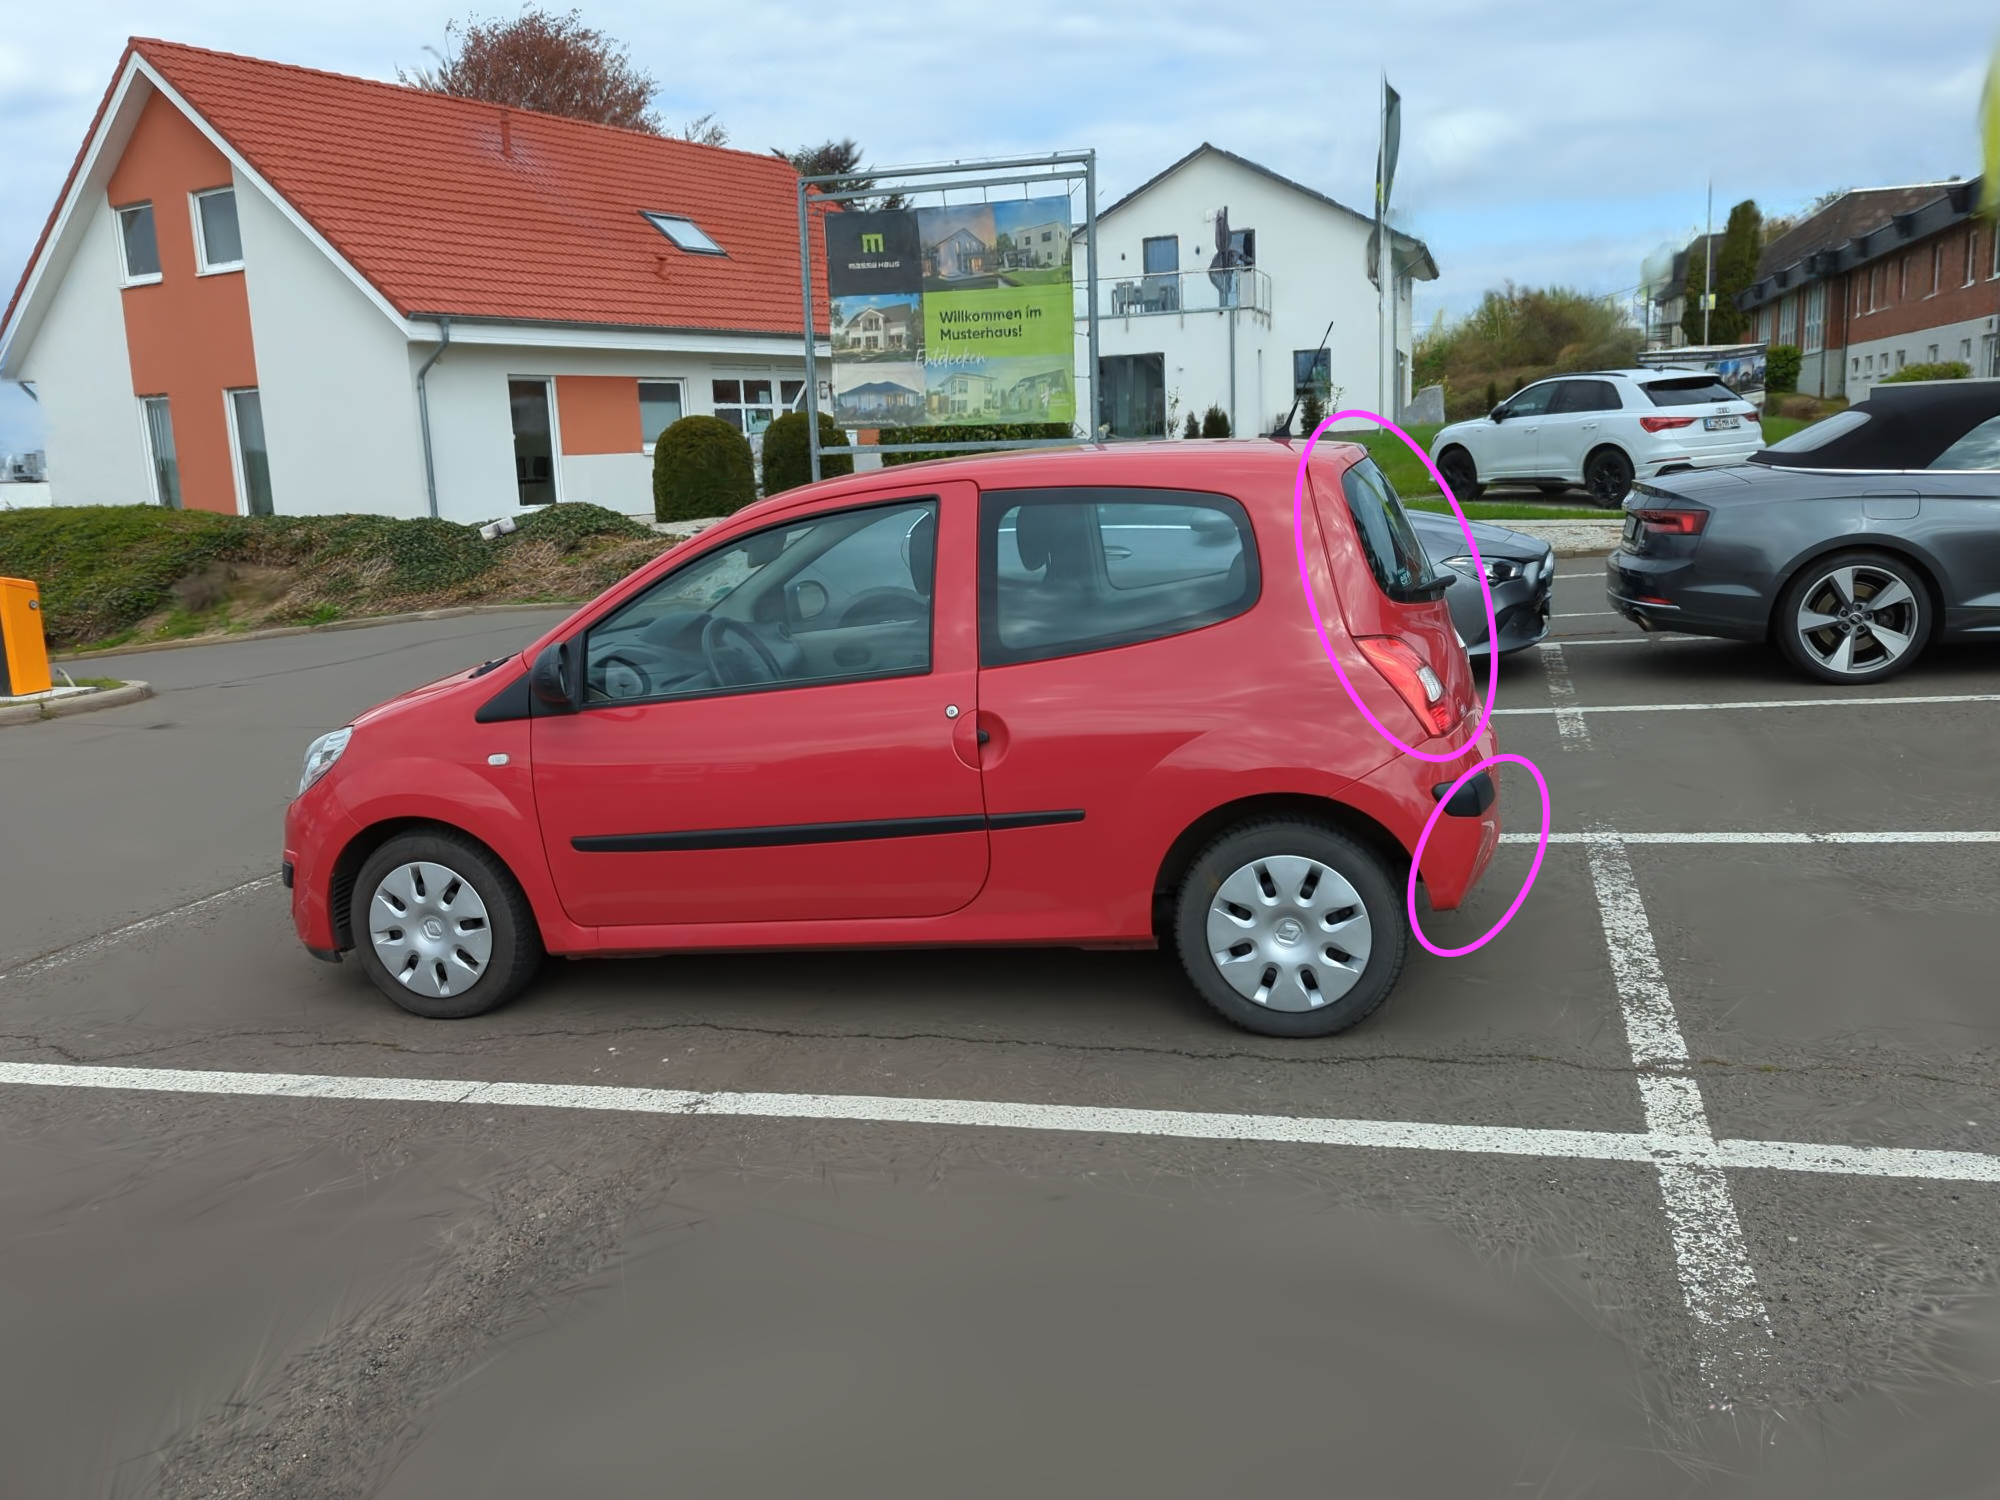
\includegraphics[width=\linewidth]{images/gaussiansplatting/00023-unstabilized.png}
    \caption{\textbf{Rendering at training location (unstabilized).}}
  \end{subfigure}
  \quad % Space between the figures
  \begin{subfigure}[b]{0.45\linewidth}
    \includegraphics[width=\linewidth]{images/gaussiansplatting/00023-stabilized.png}
    \caption{\textbf{Rendering at non-training location (stabilized).}}
  \end{subfigure}
  \caption{\textbf{Main limitation for $360^{\circ}$ spin stabilization.} While a rendering at a training location gives appealing result, moving ahead and try to render the same scene remains a challenging case that is for know unadressed.}
  \label{fig:nontraining-rendering}
\end{figure}


\section{Conclusion}

We develop in this last chapter a 3D reconstruction pipeline to perform \ac{NVS} for an industrial application. We leverage onto original \ac{GS} \citep{kerbl20233d} work to design a system that suits the specific requirements CarCutter has regarding $360^{\circ}$ spin stabilization. In this way, we extend the original \ac{GS} 3D reconstruction pipeline with three main components: a visual hull point cloud initialization, a view-dependent opacity computation and a better densification strategy. Each of these modules directly tackle a challenging issue that 3DGS was not able to deal with. First, the visual hull point cloud (that directly herits from silhouette-from-motion concept) enables to start the training process with more points on the surface of interest, the car we aim to reconstruct. Then, gaussian primitives opacity are made view-dependant through a tiny MLP. Such a network allow to better render reflective and/or transparent surfaces, such as windows in our study case. Finally, the densification strategy proposed by PixGS \citep{zhang2024pixel} has a significant impact when it comes to render tiny details and complex structure, by re-thinking the way gaussians should be cloned or splitted. Furthermore, such a novel \ac{ADC} strategy does not hurt training time as only a pixel area scaling term need to be computed. We extensively test our entire pipeline onto a single scene (that could have been one from a CarCutter customer) through different ablation studies and comparisons with a homography-based solution. One of the core limitation remain the rendering at non-training locations, \ie at stabilized positions in our case. Several artifacts can appear when the 3D scene is rendered at those unseen and out-of-distribution camera positions, and further works will try to adress this main limitation. 



